%--------------------------------------------------------------------------
% Dokumentenklasse
%--------------------------------------------------------------------------

% disable Warning for remreset Package
% \RequirePackage{silence}
% \WarningFilter{remreset}{The remreset package}

\documentclass[
	pagesize,
	fontsize=12pt,
	paper=a4,
	oneside,
   reqno
]{scrartcl}

%--------------------------------------------------------------------------
% Standardpakete 
%--------------------------------------------------------------------------
\usepackage[ngerman]{babel}               % Deutsch Silbentrennung
\usepackage[T1]{fontenc}                  % Font Type
\usepackage[utf8]{inputenc}               % Font Encoding
\usepackage{lmodern}                      % Latin Modern Font
\usepackage{csquotes}                     % Setzen von Zitaten
\usepackage{xspace}                       % setzten von Leerzeichen nach Abkürzungen
\usepackage{microtype}                    % für glattere Seitenränder
\renewcommand*\familydefault{\sfdefault}  % Serifen lose Schrift
%\renewcommand*\familydefault{\ttdefault} % Schreibmaschinenschrift

%--------------------------------------------------------------------------
% Extra Packages
%--------------------------------------------------------------------------

% Abkürzungspaket
\usepackage{acronym}

% Symbolverzeichnis
\usepackage[symbols,nogroupskip,nonumberlist,sort=use]{glossaries-extra}

\makenoidxglossaries

\glsxtrnewsymbol[description={Gewichtskraft}]{FG}{\ensuremath{F_{\mathrm{G}}}}
\glsxtrnewsymbol[description={Gewichtskraft in Bewegungsrichtung}]{FG1}{\ensuremath{F^{'}_{\mathrm{G}}}}
\glsxtrnewsymbol[description={Bewegungskraft des Schlittens}]{Fa}{\ensuremath{F_{\mathrm{a}}}}
\glsxtrnewsymbol[description={Pendelkraft}]{FP}{\ensuremath{F_{\mathrm{P}}}}
\glsxtrnewsymbol[description={Pendelkraft in Bewegungsrichtung}]{FP1}{\ensuremath{F^{'}_{\mathrm{P}}}}
\glsxtrnewsymbol[description={Reibkraft}]{Ff}{\ensuremath{F_{\mathrm{f}}}}
\glsxtrnewsymbol[description={Coulombsche Reibung}]{FC}{\ensuremath{F_{\mathrm{C}}}}
\glsxtrnewsymbol[description={Gesamtkraft}]{Fges}{\ensuremath{F_{\mathrm{ges}}}}
\glsxtrnewsymbol[description={Pendelmoment}]{MP}{\ensuremath{M_{\mathrm{P}}}}
\glsxtrnewsymbol[description={Gewichtsmoment}]{MG}{\ensuremath{M_{\mathrm{G}}}}
\glsxtrnewsymbol[description={Reibmoment}]{Mf}{\ensuremath{M_{\mathrm{f}}}}
\glsxtrnewsymbol[description={Gesamtmoment}]{Mges}{\ensuremath{M_{\mathrm{ges}}}}

% Mathe Pakete
\usepackage{amsmath}
\DeclareMathOperator{\sgn}{sgn}
\usepackage{thmtools}
\usepackage{amsfonts}
\usepackage{amssymb}
\usepackage{mathtools}
\usepackage{breqn}

% Listenumgebungen
\usepackage{listings}
\usepackage{paralist}
\usepackage{enumitem}
\usepackage{adjustbox}

% Demo Text
\usepackage{blindtext}

% Farb-Pakete
\usepackage{xcolor}
\usepackage{fancyvrb}
\usepackage{colortbl}

% Farbedefinitionen
\definecolor{htw}{RGB}{120, 184, 2}
\definecolor{ccW}{RGB}{255,255,255}
\definecolor{ccR}{RGB}{197,14,31}
\definecolor{ccG}{RGB}{113,113,113}
\definecolor{ccL}{RGB}{220,220,220}
\definecolor{ccS}{RGB}{0,0,0}
\definecolor{ccB}{RGB}{68,73,159}
\definecolor{ccD}{RGB}{0,0,80}

% Für erweiterte Tabellen
\usepackage{longtable}
\usepackage{tabularx}
\usepackage{float}
\usepackage{multirow}
\usepackage{makecell}
% \setlength{\tabcolsep}{0.5em}       % for the horizontal padding
% {\renewcommand{\arraystretch}{1.8}  % for the vertical padding
% \usepackage{ragged2e}
% \newcolumntype{R}[1]{>{\RaggedRight}p{#1}}

% Einheitenpaket
\usepackage[exponent-product = \cdot]{siunitx}
\sisetup{locale=DE}

\makeatletter
\renewcommand\@dotsep{5}
\makeatother

% Pakete für Grafiken
\usepackage{graphicx}
\usepackage{wrapfig}
\usepackage{overpic}
\usepackage{epstopdf}
\usepackage{caption}
\usepackage{subcaption}
\usepackage{rotating}
\usepackage{lscape}
% \captionsetup[subfigure]{list=true, font=normalsize, labelformat=brace, position=top} %setup für subfigure captions

% Diagramm-/Grafikerstellung
\usepackage{pstricks}
\usepackage{tikz}
\usetikzlibrary{math}
\usepackage{pgfplots}
\pgfplotsset{compat=1.5}
\usetikzlibrary{intersections,positioning,arrows,automata,calc,patterns,shapes.multipart,fit,backgrounds,decorations.pathreplacing}
\usetikzlibrary{decorations,shapes.geometric}
\usetikzlibrary{matrix,calc,angles,positioning,quotes}
% \usepackage{tikz-uml}

\usepackage{pgfkeys}
\usepackage{pgfopts}
\usepackage{ifthen}
\usepackage{xstring}
\usepackage{calc}
\usepackage{pst-plot,pst-bar,pst-node} % Balkendiagramme
\usepackage{capt-of}
\usepackage{incgraph} % Fullscreen Images
\usepackage{pdfpages} % Include external pdf pages

\usepackage{latexsym}
\usepackage{censor}
\usepackage{here}
% \StopCensoring        % Auskommentiert wird der Text entschwaerzt 
% \censor{Oszilloskop}  % Befehl zum einschwärzen
\usepackage{trfsigns}   % Transformation Symbol o---o \laplace and \Laplace
\usepackage{circuitikz}

\usepackage{multido}

% Verlinkungen im Text
\usepackage{url}
\usepackage{hyperref}
\PassOptionsToPackage{hyphens}{url}
\hypersetup{hidelinks}
\urlstyle{same}

%--------------------------------------------------------------------------
% Eigene Befehle
%--------------------------------------------------------------------------
% Test 
% \renewcommand{\thesection}{\arabic{section}} % Section startet mit 1.0 und nicht mit 0.1

%------------sectioning command-------------------
% The sectioning command one level down the hierarchy from \subsubsection is called \paragraph followed by \subparagraph
% to include this in your table of contents

% for paragraph
\setcounter{tocdepth}{4}
\setcounter{secnumdepth}{4}
% for subparagraph
\setcounter{tocdepth}{5}
\setcounter{secnumdepth}{5}

% Abkürzungen durch Kommandos setzen
\newcommand{\bspw}{bspw.\xspace}
\newcommand{\bzw}{bzw.\xspace}
\newcommand{\etc}{etc.\xspace}
\newcommand{\zB}{z.\,B.\xspace}
\newcommand{\EV}{e.\,V.\xspace}
\newcommand{\zT}{z.\,T.\xspace}
\newcommand{\iVm}{i.\,V.\,m.\xspace}
\newcommand{\idR}{i.\,d.\,R.\xspace}
\newcommand{\ihv}{i.\,H.\,v.\xspace}
\newcommand{\ua}{u.\,a.\xspace}
\newcommand{\dH}{d.\,h.\xspace}
\newcommand{\vgl}{vgl.\xspace}
\newcommand{\ca}{ca.\xspace}
\newcommand{\dV}{d.\,Verf.}
\newcommand{\RNr}{Rn.\xspace}
\newcommand{\oa}{o.\,{ä}.\xspace}
\newcommand{\vC}{v.\,Chr.\xspace}
\newcommand{\nC}{n.\,Chr.\xspace}
\newcommand{\vA}{v.\,a.\xspace}
\newcommand{\eng}{engl.\xspace}
\newcommand{\tabitem}{~~\llap{\textbullet}~~}

%------------Zitate-------------------------------
\newcommand*{\zitat}[2]{%
   \normalfont\small
   \begin{quote}
   \glqq#1\grqq \par
   #2
   \end{quote}
   \normalsize
}
\newcommand*{\zitatmitueberschrift}[3]{%
   \normalfont\small
   \begin{quote} #3
   \glqq#1\grqq \par
   #2
   \end{quote}
   \normalsize
}
\newcommand*{\zitext}[2]{%
   \glqq#1\grqq\ %
   [#2]%
}

%-----------Seitendesign--------------------------
\usepackage[width=15.5cm, height=23cm, includeheadfoot]{geometry}
\geometry{paper=a4paper}
% \usepackage[left=6cm,right=1cm,top=1.5cm, bottom=1cm, includeheadfoot]{geometry}
% \newgeometry{oneside}
% \setlength{\voffset}{0cm}
\setlength{\headheight}{1.1\baselineskip} % increase headheight
\setlength{\footheight}{28.99998pt}       % increase foodheight
\setlength{\parindent}{0cm}               % Einrücken nach \newline
\setlength{\footskip}{86pt}               % Move Footer down
% \setlength{\topmargin}{0cm}
% \setlength{\marginparsep}{0.5cm}
% \setlength{\marginparwidth}{1.5cm}
% \setlength{\textwidth}{16cm}
% \setlength{\textheight}{23cm}
% \setlength{\oddsidemargin}{1cm}
% \setlength{\evensidemargin}{2cm}

%----------Kopf & Fußzeile------------------------
% \usepackage[headsepline,footsepline]{scrpage2}
\usepackage[headsepline]{scrlayer-scrpage}
\pagestyle{scrheadings}
\clearpairofpagestyles
\ihead{\headmark}
\automark{section}
\chead{}
\ohead{
\includegraphics[scale=0.09]{Bilder/HTWLogoKopfzeile.png} \nocite{HTWklein}}
\ifoot{Sebastian Richter\\ Aaron Zielstorff}
\cfoot{\pagemark}
\ofoot{VA1 Moderne Methoden\\ der Regelungstechnik}

%--------------------------------------------------------------------------
% Beginn des Dokuments
%--------------------------------------------------------------------------
\begin{document}

%----------Deckblatt----------------------------- 
\begin{titlepage}
   \pagestyle{empty} % setzt Pagestyle-Befehl

   % HTW Logo
   \begin{flushright}
   
\includegraphics[scale=.07]{Bilder/LogoHTWBerlin.png}  \nocite{HTWgross}
   \end{flushright}

   \vspace{1cm}

   % Titel
   \begin{center}
      \Huge{\textbf{Inverses Pendel: Moderne Methoden der Regelungstechnik (VA1)}} \\
   \end{center}

   \vspace{3cm}

   % Name
   \begin{flushleft}
      \begin{tabular}{l c l }
         \textbf{Name: }&\hspace{1 cm} &\textbf{Matrikelnummer:} \\
         Sebastian Richter  & & 572906 \\
         Aaron Zielstorff   & & 567183 \\
      \end{tabular}
   \end{flushleft}

   \vspace{1cm}

   % Daten
   \begin{tabular}{l l}
      \textbf{Fachbereich:}   & FB1                                                 \\
      \textbf{Studiengang:}   & M.\xspace Elektrotechnik                            \\
      \textbf{Fachsemester:}  & 2.\xspace FS                                        \\
      \textbf{Fach:}          & VA1 Moderne Methoden der Regelungstechnik           \\
      \textbf{Dozent:}        & Prof.\xspace Dr.\xspace -Ing.\xspace Horst Schulte  \\
      \textbf{Abgabe am:}     & 19.\xspace Juli 2022                                \\ 
   \end{tabular}
\end{titlepage}
\clearpage

%--------Inhaltsverzeichnis-----------------------
\renewcommand{\contentsname}{Inhaltsverzeichnis}
\tableofcontents
\clearpage

%--------Abbildungsverzeichnis--------------------
\renewcommand{\listfigurename}{Abbildungsverzeichnis}
\renewcommand*{\figurename}{Abb.}
\listoffigures
% \clearpage

%--------Tabellenverzeichnis----------------------
\renewcommand*{\listtablename}{Tabellenverzeichnis}
\renewcommand*{\tablename}{Tab.}
\listoftables
\clearpage

%----------Symbolverzeichnis----------------------
% \printnoidxglossary[type=symbols,style=long,title={Symbolverzeichnis}]
% \clearpage

%---------Kapitel/Text----------------------------

\section{Einführung in die Regelaufgabe}

Ziel des Beleges ist die Modellierung und Regelung eines inversen Pendels, welches auf einem durch einen Motor bewegten Schlitten befestigt ist. Über die Regelung soll es möglich sein das Pendel in der instabilen Ruhelage aufrecht stehen zu lassen. Dies soll ausschließlich über die Bewegung des Schlittens möglich sein. Es gelten folgende Voraussetzungen für das System:

\begin{itemize}
    \item Das Pendel ist frei gelagert.
    \item Der Motor (Synchronmaschine) ist momentengeregelt.
    \item Die Position und Geschwindigkeit des Schlittens werden erfasst.
    \item Der Winkel, aber nicht die Winkelgeschwindigkeit, des Pendels wird gemessen.
\end{itemize}

Es werden folgende Einschränkungen festgelegt:

\begin{itemize}
    \item Der Schlitten darf den Arbeitsbereich nicht verlassen.
    \item Es soll ein Zustandsregler mit vier Zuständen verwendet werden.
    \item Für die Ermittlung der Winkelgeschwindigkeit ist eine Rekonstruktion über einen Beobachter notwendig.
\end{itemize}

Für die Umsetzung der Aufgabe sind nachfolgende Modellparameter gegeben:

\begin{table}[H]
    \centering
    \begin{tabular}{lll}
        \hline
        Symbol   & Parameter                           & Wert                                   \\ \hline
        $l$      & Länge des Pendels                   & $\SI{40}{cm}$                          \\
        $m$      & Gewicht des Pendels                 & $\SI{260}{g}$                          \\
        $M$      & Gewicht des gesamten Schlittens     & $\SI{3}{kg}$                           \\
        $F_{\mathrm{c}}$    & Coulombsche Reibung                 & $\SI{16}{\frac{kg \cdot m}{s^2}}$      \\
        $d$      & Dämpfungskoeffizient des Schlittens & $\SI{7}{\frac{kg}{s}}$                 \\
        $d_{\mathrm{Mf}}$ & Lagerreibung                        & $\SI{0.00095}{\frac{kg \cdot m}{s^2}}$ \\ \hline
    \end{tabular}
    \caption{Modellparameter des Inversen Pendels}
    \label{tab:my-table1}
\end{table}

\begin{figure}[H]
   \centering
   \fbox{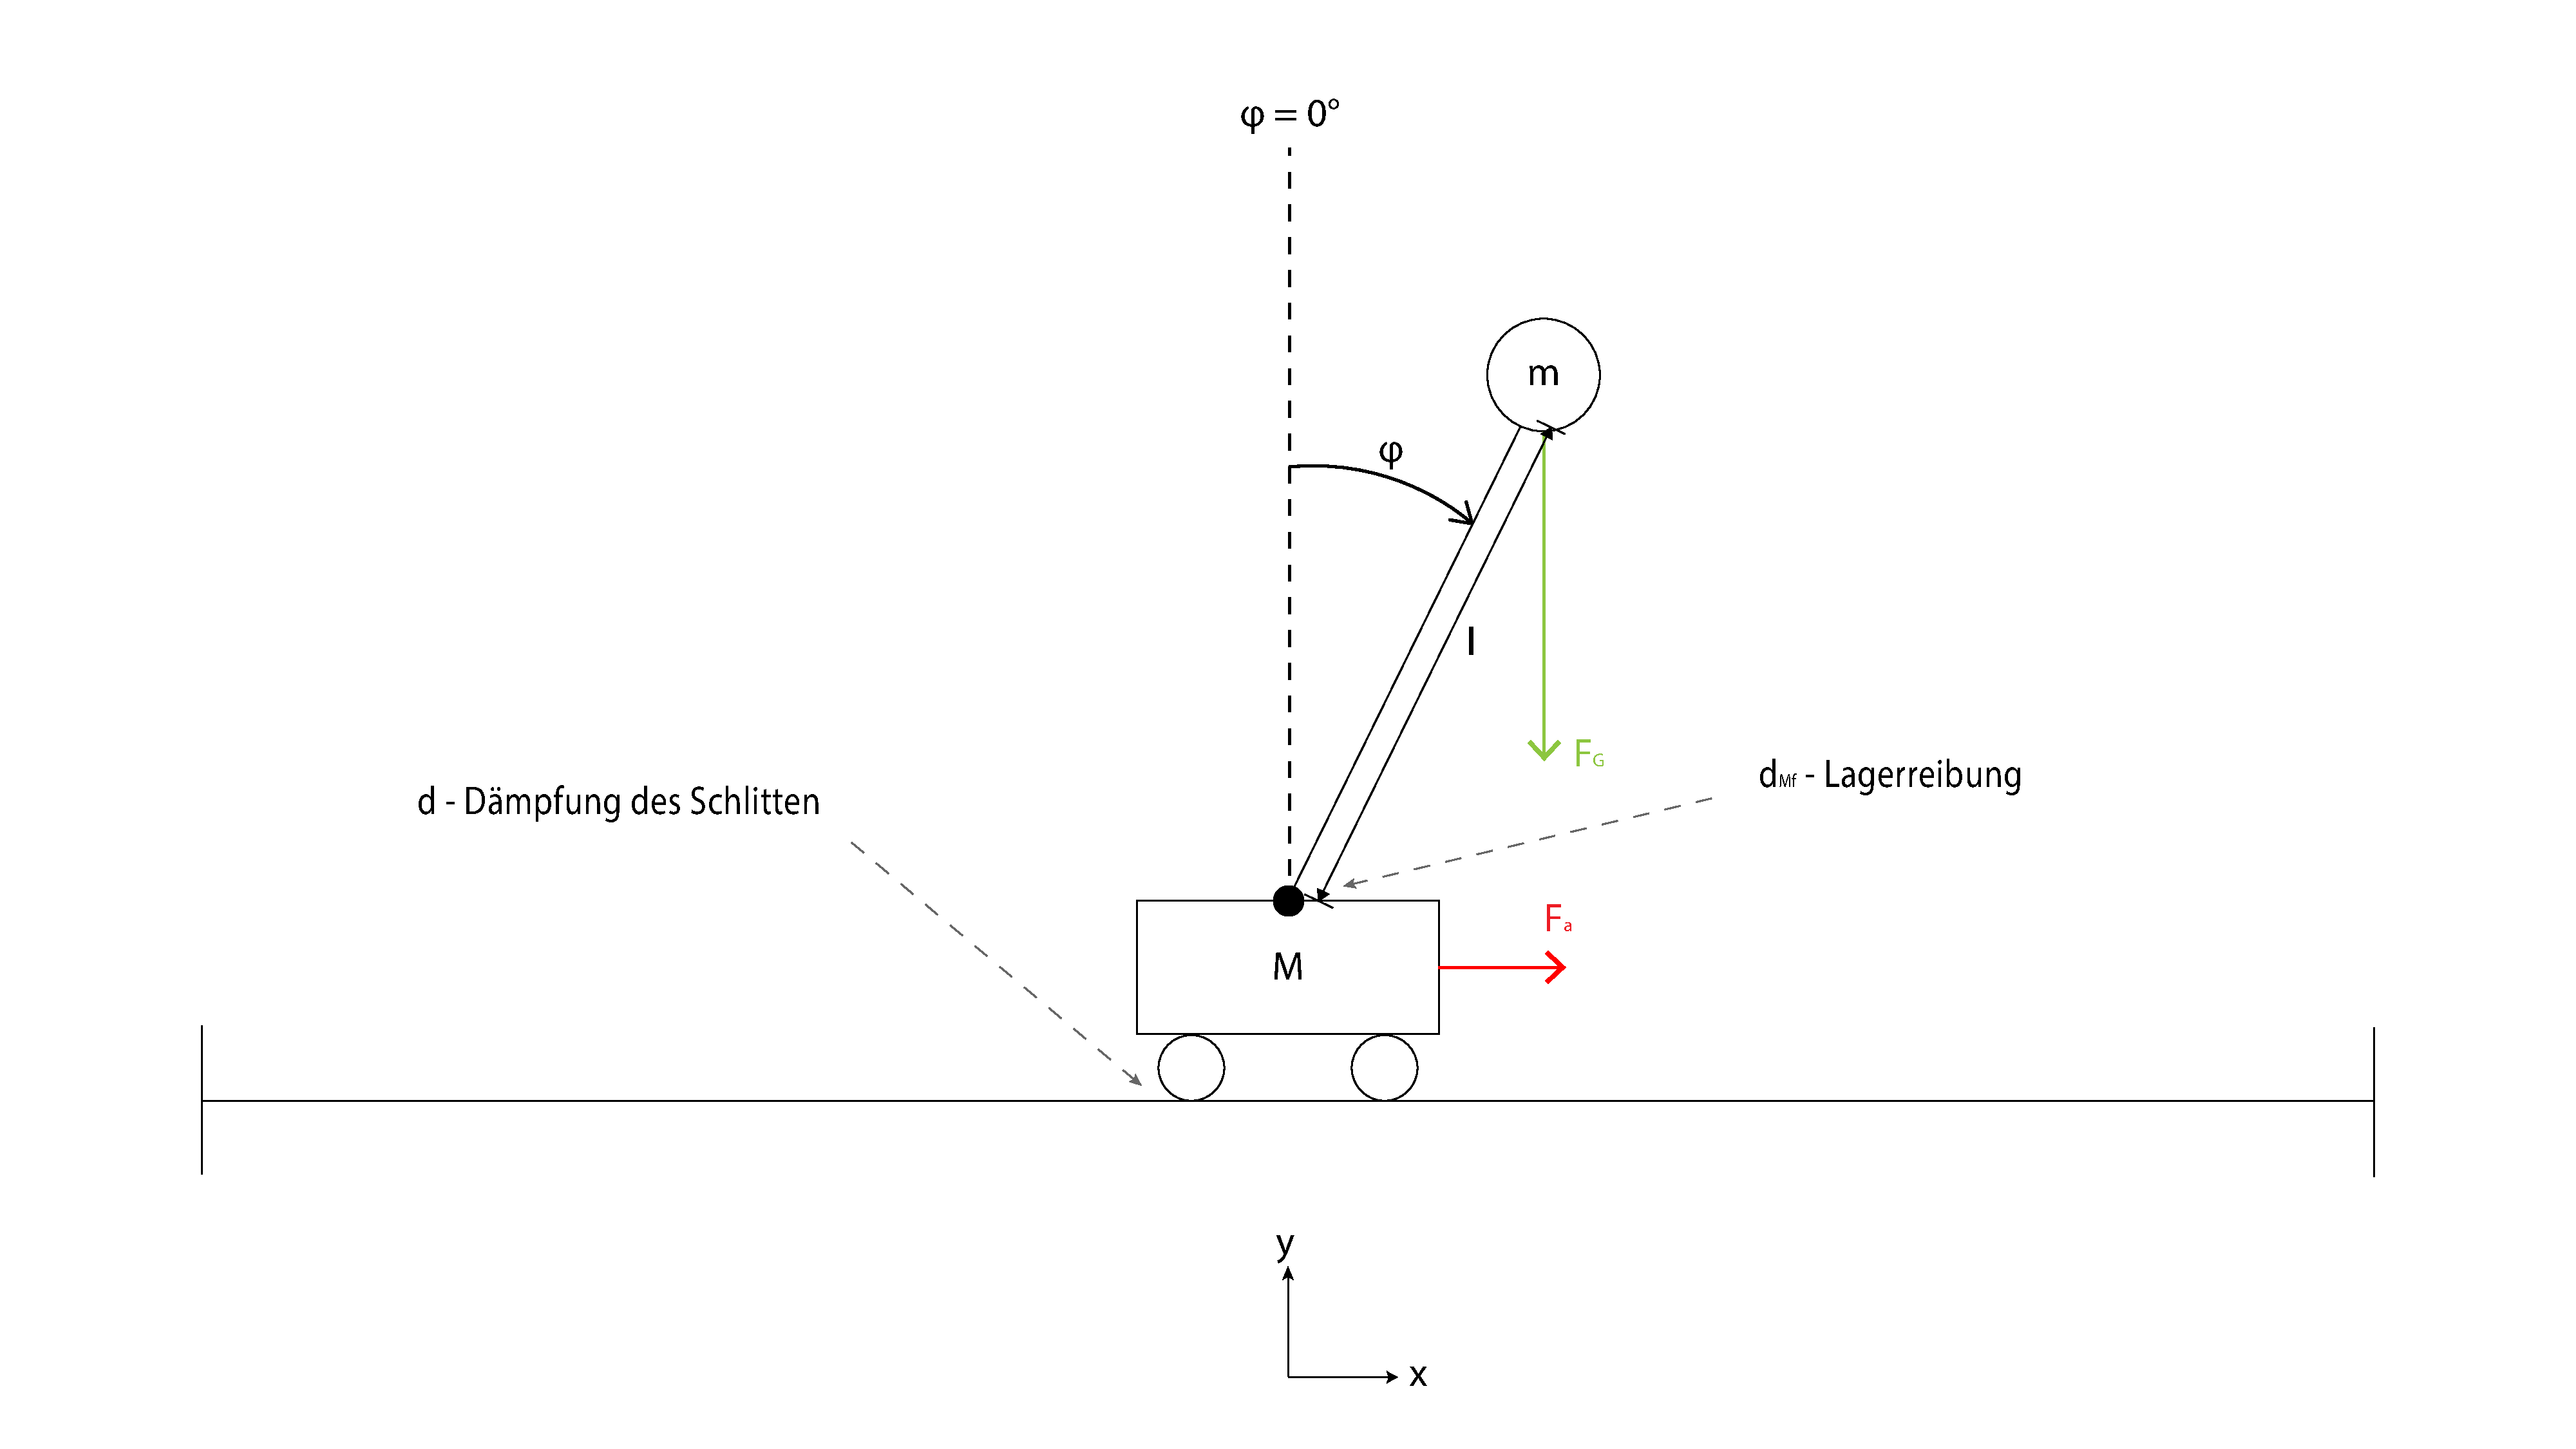
\includegraphics[width=1.0\textwidth]{Bilder/Inverses_Pendel_Skizze.pdf}}
   \caption[Skizze des Aufbaus der Regelaufgabe]{Skizze des Aufbaus der Regelaufgabe Inverses Pendel mit Darstellung der Einwirkenden Kräfte und Momente}
   \label{fig:Bild1}
\end{figure}

\clearpage

\section{Modellierung: Energiemethode nach Lagrange}

\subsection{Ansatz}

Die nachfolgende Gleichung zeigt den Lagrange Ansatz unter Berücksichtigung der dissipativen Funktion. Diese besagt in Erweiterung zu der Lagrange-Formulierung, dass Energie in einem Vorgang in Wärme umgewandelt wird. Mit Hilfe der dissipativen Funktion können Reibungsverluste bei der Energiemethode nach Lagrange berücksichtigt werden.

\begin{align} \label{eq:Gleichung1}
    \frac{d}{dt} \left(\frac{\partial L}{\partial \dot{q_{\mathrm{i}}}}\right) - \frac{\partial L}{\partial q_{\mathrm{i}}} + \frac{\partial D}{\partial \dot{q_{\mathrm{i}}}} = F_{\mathrm{i}}
\end{align}

\subsection{Freiheitsgrade und Zwangsbedingungen}

In \autoref{fig:Bild1} sind zwei Massepunkte im $\mathbb{R}^2$ zu erkennen. Somit gilt grundsätzlich:
\begin{itemize}
    \item 2 Punkte: 4 Freiheitsgrade (FHG)
\end{itemize}

Das inverse Pendel besitzt jedoch auch zwei Zwangsbedingungen, die wie folgt formuliert werden können:

\begin{itemize}
    \item Der Wagen kann sich nur horizontal bewegen: \\ $y_{\mathrm{M}} = 0$
    \item Die Masse $m$ am Ende des Pendels ist mit dem Wagen gekoppelt: \\ $(y_{\mathrm{M}} - y_{\mathrm{m}})^2 + (x_{\mathrm{M}} - x_{\mathrm{m}})^2 = l^2$
\end{itemize}

Somit bleiben am Ende noch zwei Freiheitsgrade (FHG) übrig.

\subsection{Generalisierte Koordinaten}

Aus den verbliebenen Freiheitsgraden können nun die beiden generalisierten Koordinaten abgeleitet werden.

\begin{itemize}
    \item $q_{\mathrm{1}} = x_{\mathrm{M}}$
    \item $q_{\mathrm{2}} = \varphi$
\end{itemize}

\subsection{Berechnung der kinetischen und potentiellen Energie}

Der Ansatz zur Berechnung einer kinetischen Energie ist nachfolgend gezeigt.

\begin{align}\label{eq:Gleichung2}
    E_{\mathrm{kin}} = \frac{1}{2} \cdot m \cdot v^2
\end{align}

Zu berücksichtigen ist, dass beide Massen ($m$ und $M$) eine kinetische Energie besitzen (\autoref{eq:Gleichung3} und \autoref{eq:Gleichung4}).

\begin{align}
    E_{\mathrm{kin}} &= \frac{1}{2} \cdot M \cdot \dot{x}_{\mathrm{M}}^2 + \frac{1}{2} \cdot m \cdot v_{\mathrm{m}}^2 \label{eq:Gleichung3} \\
    E_{\mathrm{kin}} &= \frac{1}{2} \cdot M \cdot \dot{x}_{\mathrm{M}}^2 + \frac{1}{2} \cdot m \cdot \left(\dot{x}_{\mathrm{m}}^2 + \dot{y}_{\mathrm{m}}^2\right) \label{eq:Gleichung4}
\end{align} \\

Weiter gilt:

\begin{align*}
    x_{\mathrm{m}} &= x_{\mathrm{M}} + l \cdot \sin({\varphi}) \\
    y_{\mathrm{m}} &= l \cdot \cos({\varphi}) \\
    \dot{x_{\mathrm{m}}} &= \dot{x_{\mathrm{M}}} + l \cdot \dot{\varphi} \cdot \cos{\varphi} \\
    \dot{y_{\mathrm{m}}} &= -l \cdot \dot{\varphi} \cdot \sin({\varphi})
\end{align*}

Daraus resultiert:

\begin{dmath*}
    E_{\mathrm{kin}} = \frac{1}{2} \cdot M \cdot \dot{x}_{\mathrm{M}}^2 + \frac{1}{2} \cdot m \cdot \left(\left(\dot{x}_{\mathrm{M}} + l \cdot \dot{\varphi} \cdot \cos({\varphi})\right)^2 + \left( -l \cdot \dot{\varphi} \cdot \sin({\varphi})\right)^2\right) \\
    = \frac{1}{2} \cdot M \cdot \dot{x}_{\mathrm{M}}^2 + \frac{1}{2} \cdot m \cdot \left(\dot{x}_{\mathrm{M}}^2 + 2 \cdot \dot{x}_{\mathrm{M}} \cdot l \cdot \dot{\varphi} \cdot \cos({\varphi}) + l^2 \cdot \dot{\varphi}^2 \cdot \cos^2(\varphi) + l^2 \cdot \dot{\varphi}^2 \cdot \sin^2(\varphi)\right) \\
    = \frac{1}{2} \cdot M \cdot \dot{x}_{\mathrm{M}}^2 + \frac{1}{2} \cdot m \cdot \dot{x}_{\mathrm{M}}^2 + m \cdot \dot{x}_{\mathrm{M}} \cdot l \cdot \dot{\varphi} \cdot \cos({\varphi}) + \frac{1}{2} \cdot m \cdot l^2 \cdot \dot{\varphi}^2 \cdot \cos^2(\varphi) + \frac{1}{2} \cdot m \cdot l^2 \cdot \dot{\varphi}^2 \cdot \sin^2(\varphi)
\end{dmath*}

Durch das Zusammenfassen der vorangegangenen Beziehung folgt die \autoref{eq:Gleichung5} für die gesamte kinetische Energie des Systems.

\begin{align} \label{eq:Gleichung5}
    E_{\mathrm{kin}} = \frac{1}{2} \cdot \dot{x}_{\mathrm{M}}^2 \cdot (M + m) + \frac{1}{2} \cdot m \cdot \left( 2 \cdot \dot{x}_{\mathrm{M}} \cdot l \cdot \dot{\varphi} \cdot \cos({\varphi}) + l^2 \cdot \dot{\varphi}^2\right)
\end{align}

Ausschließlich die Masse $m$ am Pendelende besitzt eine für den Lagrange-Formalismus relevante potentielle Energie (\autoref{eq:Gleichung6}).

\begin{align}
    E_{\mathrm{pot}} &= m \cdot g \cdot h \nonumber \\
    E_{\mathrm{pot}} &= m \cdot g \cdot y_{\mathrm{m}} \nonumber \\
    E_{\mathrm{pot}} &= m \cdot g \cdot l \cdot \cos({\varphi}) \label{eq:Gleichung6}
\end{align}

\subsection{Herleitung der Bewegungsgleichungen}

Die Lagrange-Funktion wird aus der Differenz der kinetischen und der potentiellen Energie berechnet (\autoref{eq:Gleichung7}).

\begin{align} 
        L &= E_{\mathrm{kin}} - E_{\mathrm{pot}}  \label{eq:Gleichung7} \\ 
        L &= \frac{1}{2} \cdot \dot{x}_{\mathrm{M}}^2 \cdot (M + m) + \frac{1}{2} \cdot m \cdot \left( 2 \cdot \dot{x}_{\mathrm{M}} \cdot l \cdot \dot{\varphi} \cdot \cos({\varphi}) + l^2 \cdot \dot{\varphi}^2\right) - m \cdot g \cdot l \cdot \cos({\varphi}) \label{eq:Gleichung8}
\end{align}

Im ersten Schritt wird die Bewegungsgleichung des Wagens hergeleitet. Dafür wird zunächst \autoref{eq:Gleichung8} nach der ersten zeitlichen Ableitung der generalisierten Koordinate $x_{\mathrm{M}}$ partiell differenziert:

\begin{align}\label{eq:Gleichung9}
    \frac{\partial L}{\partial \dot{x}_{\mathrm{M}}} = (M + m) \cdot \dot{x}_{\mathrm{M}} + m \cdot l \cdot \dot{\varphi} \cdot \cos(\varphi)
\end{align}

Die vorangegangene Gleichung wird zeitlich differenziert:

\begin{align}\label{eq:Gleichung10}
    \frac{d}{dt}\left(\frac{\partial L}{\partial \dot{x}_{\mathrm{M}}}\right) = (M + m) \cdot \ddot{x}_{\mathrm{M}} + m \cdot l \cdot \left(\ddot{\varphi} \cdot \cos(\varphi) - \dot{\varphi}^2 \cdot \sin(\varphi) \right)
\end{align}

Im zweiten Schritt wird die Lagrange-Funktion nach der generalisierten Koordinate $x_{\mathrm{M}}$ abgeleitet.

\begin{align}\label{eq:Gleichung11}
    \frac{\partial L}{\partial x_{\mathrm{M}}} = 0
\end{align}

Abschließend wird die dissipative Funktion nach der 1. Ableitung der generalisierten Koordinate $x_{\mathrm{M}}$ differenziert.

\begin{align}\label{eq:Gleichung12}
    \frac{\partial D}{\partial \dot{x_{\mathrm{M}}}} = d \cdot \dot{x_{\mathrm{M}}}
\end{align}

Durch das Einsetzen der \autoref{eq:Gleichung9} bis \autoref{eq:Gleichung12} in den Ansatz aus \autoref{eq:Gleichung1} resultiert die vollständige Bewegungsgleichung des Wagens.

\begin{align}\label{eq:Gleichung13}
    (M + m) \cdot \ddot x_{\mathrm{M}} + m \cdot l \cdot \left( \ddot \varphi \cdot \cos({\varphi}) - \dot \varphi^2 \cdot \sin({\varphi})\right) + d \cdot \dot x_{\mathrm{M}} = F_{\mathrm{a}}
\end{align}

Analog wird die Bewegungsgleichung des Pendels entwickelt. Hierbei wird zunächst \autoref{eq:Gleichung8} nach der 1. Ableitung der generalisierten Koordinate $\varphi$ partiell differenziert.

\begin{align}\label{eq:Gleichung14}
    \frac{\partial L}{\partial \dot{\varphi}} = m \cdot l \cdot \dot{x}_{\mathrm{M}} \cdot \cos(\varphi) + m \cdot l^2 \cdot \dot{\varphi}
\end{align}

Die vorangegangene Gleichung wird nach der Zeit abgeleitet:

\begin{align}\label{eq:Gleichung15}
    \frac{d}{dt}\left(\frac{\partial L}{\partial \dot{\varphi}}\right) = m \cdot l \cdot \left(\ddot{x}_{\mathrm{M}} \cdot  \cos(\varphi) - \dot{x}_{\mathrm{M}} \cdot \sin(\varphi) \cdot \dot{\varphi}\right) + m \cdot l^2 \cdot \ddot{\varphi}
\end{align}

Als nächstes wird für die Bewegungsgleichung des Pendels die Lagrange-Funktion nach der generalisierten Koordinate $\varphi$ abgeleitet:

\begin{align}\label{eq:Gleichung16}
    \frac{\partial L}{\partial \varphi} = -m \cdot l \cdot \dot{\varphi} \cdot \dot{x}_{\mathrm{M}} \cdot \sin(\varphi) + m \cdot g \cdot l \cdot \sin(\varphi)
\end{align}

Abschließend wird die dissipative Funktion analog nach der 1. Ableitung der generalisierten Koordinate $\varphi$ differenziert:

\begin{align}\label{eq:Gleichung17}
    \frac{\partial D}{\partial \dot{\varphi}} = d_{\mathrm{Mf}} \cdot \dot{\varphi}
\end{align}

Über das Anwenden von \autoref{eq:Gleichung1} folgt die Bewegungsgleichung des Pendels zu:

\begin{align}\label{eq:Gleichung18}
    \ddot{x}_{\mathrm{M}} \cdot \cos(\varphi) + l \cdot \ddot{\varphi} - g \cdot \sin(\varphi) + \frac{d_{\mathrm{Mf}} \cdot \dot{\varphi}}{m \cdot l} = 0
\end{align}

\section{Nichtlineares Zustandsraummodell}

\subsection{Umformungen}

Zum Aufstellen des nichtlinearen Zustandsraummodells werden die \autoref{eq:Gleichung13} und \autoref{eq:Gleichung18} nach den höchsten Ableitungen $\ddot x_{\mathrm{M}}$ und $\ddot \varphi$ umgestellt.

\begin{align}
    \ddot x_{\mathrm{M}} &= \frac{-d_{\mathrm{Mf}} \cdot \dot \varphi -m \cdot l^2 \cdot \ddot \varphi + m \cdot g \cdot l \cdot \sin({\varphi})}{m \cdot l \cdot \cos({\varphi})} \label{eq:Gleichung19} \\
    \ddot \varphi &= \frac{F_{\mathrm{a}} - (M+m) \cdot \ddot x_{\mathrm{M}} + m \cdot l \cdot \dot \varphi^2 \cdot \sin({\varphi}) -d \cdot \dot x_{\mathrm{M}}}{m \cdot l \cdot \cos({\varphi})} \label{eq:Gleichung20}
\end{align}

Beide Gleichungen sind über die Wagenbeschleunigung $\ddot x_{\mathrm{M}}$ und der Winkelbeschleunigung $\ddot \varphi$ miteinander verkoppelt. Durch das gegenseitige Einsetzen werden die Abhängigkeiten eliminiert.

\begin{align}
    \ddot x_{\mathrm{M}} &= \frac{-d_{\mathrm{Mf}} \cdot \dot \varphi -m \cdot l^2 \cdot \left( \frac{F_{\mathrm{a}} - (M+m) \cdot \ddot x_{\mathrm{M}} + m \cdot l \cdot \dot \varphi^2 \cdot \sin({\varphi}) -d \cdot \dot x_{\mathrm{M}}}{m \cdot l \cdot \cos({\varphi})} \right) + m \cdot g \cdot l \cdot \sin({\varphi})}{m \cdot l \cdot \cos({\varphi})} \label{eq:Gleichung21} \\
    \ddot \varphi &= \frac{F_{\mathrm{a}} - (M+m) \cdot \left( \frac{-d_{\mathrm{Mf}} \cdot \dot \varphi -m \cdot l^2 \cdot \ddot \varphi + m \cdot g \cdot l \cdot \sin({\varphi})}{m \cdot l \cdot \cos({\varphi})} \right) + m \cdot l \cdot \dot \varphi^2 \cdot \sin({\varphi}) -d \cdot \dot x_{\mathrm{M}}}{m \cdot l \cdot \cos({\varphi})} \label{eq:Gleichung22}
\end{align}

\subsection{Zustandsraumdarstellung (nichtlinear)}

Das zu untersuchende System weist vier Zustände auf, welche in Form eines Zustandsvektors $\underline{x}$ erfasst werden. Die Dokumentation der zeitlichen Ableitungen erfolgt im Vektor der Zustandsänderungen $\dot{\underline{x}}$. Der Eingangsvektor $\underline{u}$ gleicht der Eingangskraft des Systems $F_{\mathrm{a}}$.
\\\\Eingangsvektor:
\begin{align}\label{eq:Gleichung23}
    \underline{u} &= F_{\mathrm{a}}
\end{align}

Zustandsvektor:
\begin{align}
    \underline{x} &=
    \begin{bmatrix}\label{eq:Gleichung24}
        x_{\mathrm{1}} \\
        x_{\mathrm{2}} \\
        x_{\mathrm{3}} \\
        x_{\mathrm{4}}
    \end{bmatrix} =
    \begin{bmatrix}
        \varphi         \\
        \dot \varphi    \\
        x_{\mathrm{M}}  \\
        \dot x_{\mathrm{M}}
    \end{bmatrix}
\end{align}

Vektor der Zustandsänderungen:
\begin{align}\label{eq:Gleichung25}
    \dot{\underline{x}} &=
    \begin{bmatrix}
        \dot x_{\mathrm{1}} \\
        \dot x_{\mathrm{2}} \\
        \dot x_{\mathrm{3}} \\
        \dot x_{\mathrm{4}}
    \end{bmatrix} =
    \begin{bmatrix}
        \dot{\varphi}           \\
        \ddot{\varphi}          \\
        \dot{x}_{\mathrm{M}}    \\
        \ddot{x}_{\mathrm{M}}
    \end{bmatrix}
\end{align}

Mithilfe der \autoref{eq:Gleichung23} bis \autoref{eq:Gleichung25}, durch das Einsetzen in \autoref{eq:Gleichung21} und \autoref{eq:Gleichung22}, dem Zusammenfassen und Umstellen nach $\ddot x_{\mathrm{M}}$ und $\ddot \varphi$ folgt das nichtlineare Zustandsraummodell aus \autoref{eq:Gleichung14}.

\begin{align}\label{eq:Gleichung26}
    \dot{\underline{x}} &=
    \begin{bmatrix}
        x_2 \\
        \frac{\left(\frac{F_{\mathrm{a}} - g \cdot \tan(x_{\mathrm{1}}) \cdot (M + m) - d \cdot x_{\mathrm{4}}}{m \cdot l \cdot \cos(x_{\mathrm{1}})} + d_{\mathrm{Mf}} \cdot x_{\mathrm{2}} \cdot \left(\frac{M}{m^2 \cdot l^2 \cdot \cos^2(x_{\mathrm{1}})} + \frac{1}{m \cdot l^2 \cdot \cos^2(x_{\mathrm{1}})}\right) + x_{\mathrm{2}}^2 \cdot \tan(x_{\mathrm{1}})\right)}{\left(1 - \frac{1}{\cos^2(x_{\mathrm{1}})} - \frac{M}{m \cdot \cos^2(x_{\mathrm{1}})}\right)} \\
        x_{\mathrm{4}} \\
        \frac{\left(g \cdot \tan(x_{\mathrm{1}}) - \frac{F_{\mathrm{a}}}{m \cdot \cos^2(x_{\mathrm{1}})} + \frac{d \cdot x_{\mathrm{4}}}{m \cdot \cos^2(x_{\mathrm{1}})} - \frac{l \cdot x_{\mathrm{2}}^2 \cdot \tan(x_{\mathrm{1}})}{\cos(x_{\mathrm{1}})} - \frac{d_{\mathrm{Mf}} \cdot x_{\mathrm{2}}}{m \cdot l \cdot \cos(x_{\mathrm{1}})}\right)}{\left(1 - \frac{(M + m)}{m \cdot \cos^2(x_{\mathrm{1}})}\right)}
    \end{bmatrix}
\end{align}

\clearpage

\section{Linearisiertes Zustandsraummodell}

\subsection{Linearisierungsvorschrift}
Das Verhalten des nichtlinearen Systems ist für große Änderungen des Eingangssignals nicht vorhersehbar. Um dennoch Aussagen über das Systemverhalten treffen zu können, wird das nichtlineare Zustandsraummodell mithilfe der Taylorreihenentwicklung um eine Ruhelage ($\underline{x}^{*}$) linearisiert. Die nichtlinearen Restglieder $\underline{R}(\Delta{\underline{x}^2}, \Delta{\underline{u}^2})$ werden zu Null angenommen.
Durch die Linearisierung wird das Systemverhalten für kleine Änderungen um die Ruhelage kontrollierbar.\\
\\Taylorreihenentwicklung für Linearisierung:

\begin{align}\label{eq:Gleichung27}
    \begin{split}
        \dot{\underline{x}}^{*}+\Delta{\dot{\underline{x}}} &=\underline{f}(\underline{x}^{*}+\Delta{\underline{x}},\underline{u}^{*}+\Delta{\underline{u}})\\
        &=\underline{f}(\underline{x}^{*},\underline{u}^{*})+\left[\frac{\partial f_{\mathrm{i}}}{\partial x_{\mathrm{j}}}\right]_{(\underline{x}^{*}, \underline{u}^{*})}\cdot\Delta{\underline{x}}+\left[\frac{\partial f_{\mathrm{i}}}{\partial u_{\mathrm{j}}}\right]_{(\underline{x}^{*},\underline{u}^{*})}\cdot\Delta{\underline{u}}+\underline{R}(\Delta{\underline{x}^2}, \Delta{\underline{u}^2})
    \end{split}
\end{align}

Durch die Annahme über das Verhalten der nichtlinearen Restglieder folgt die Struktur des linearen Zustandraummodells aus \autoref{eq:Gleichung16}.

\begin{align}\label{eq:Gleichung28}
    \begin{split}
        \Delta\dot{\underline{x}} &= \left[\frac{\partial f_{\mathrm{i}}}{\partial x_{\mathrm{j}}}\right]_{(\underline{x}^{*}, \underline{u}^{*})}\cdot\Delta{\underline{x}}+\left[\frac{\partial f_{\mathrm{i}}}{\partial u_{\mathrm{j}}}\right]_{(\underline{x}^{*},\underline{u}^{*})}\cdot\Delta{\underline{u}}\\   
        \Delta{\underline{y}} &= \left[\frac{\partial h_{\mathrm{i}}}{\partial x_{\mathrm{j}}}\right]_{(\underline{x}^{*}, \underline{u}^{*})}\cdot\Delta{\underline{x}}+\left[\frac{\partial h_{\mathrm{i}}}{\partial u_{\mathrm{j}}}\right]_{(\underline{x}^{*},\underline{u}^{*})}\cdot\Delta{\underline{u}}
    \end{split}
\end{align}

 Allgemein gefasst, wird das lineare Zustandsraummodell folgendermaßen dargestellt:

\begin{align}\label{eq:Gleichung29}
    \begin{split}
        \dot{\underline{x}} &= A\cdot\underline{x}+B\cdot\underline{u}\\
        \underline{y} &= C\cdot\underline{x}+D\cdot\underline{u}
    \end{split}
\end{align}

\subsection{Stabile und instabile Ruhelage}
Um das linearisierte Zustandsraummodell zu erhalten, werden die einzelnen Gleichungen des nichtlinearen Zustandsraummodells aus \autoref{eq:Gleichung26} nach den Zuständen $x_{\mathrm{1}}$ bis $x_{\mathrm{4}}$, sowie dem Eingang $F_{\mathrm{a}}$ partiell abgeleitet und die entsprechende Ruhelage eingesetzt. Folgende Ruhelagen werden betrachtet:\\
Hängendes Pendel:
\begin{align}\label{eq:Gleichung30}
    \begin{split}
        \underline{x}_{\mathrm{1}}^{*}=
        \begin{bmatrix}
            x_{\mathrm{1}}^{*}\\
            x_{\mathrm{2}}^{*}\\
            x_{\mathrm{3}}^{*}\\
            x_{\mathrm{4}}^{*}
        \end{bmatrix}=
        \begin{bmatrix}
            Pi\\
            0\\
            0\\
            0
        \end{bmatrix}
    \end{split}
\end{align}

Stehendes Pendel:
\begin{align}\label{eq:Gleichung31}
    \begin{split}
        \underline{x}_{\mathrm{2}}^{*}=
        \begin{bmatrix}
            x_{\mathrm{1}}^{*}\\
            x_{\mathrm{2}}^{*}\\
            x_{\mathrm{3}}^{*}\\
            x_{\mathrm{4}}^{*}
        \end{bmatrix}=
        \begin{bmatrix}
            0\\
            0\\
            0\\
            0
        \end{bmatrix}
    \end{split}
\end{align}

\subsection{Zustandsraumdarstellung (linear)}

Die linearisierten Zustandsraummodelle unter Berücksichtigung der Ruhelagen resultieren zu:\\
\\Hängendes Pendel:
\begin{align}\label{eq:Gleichung32}
    \begin{split}
        \Delta{\dot{\underline{x}}}&=
        \begin{bmatrix}
            0 & 1 & 0 & 0 \\
            -26.6505 & -0.0248 & 0 & -5.8333 \\
            0 & 0 & 0 & 1 \\
            -0.8502 & -7.916\cdot10^-4 & 0 & -2.333
        \end{bmatrix}\cdot
        \begin{bmatrix}
            \Delta{x_{\mathrm{1}}} \\ \Delta{x_{\mathrm{2}}} \\ \Delta{x_{\mathrm{3}}} \\ \Delta{x_{\mathrm{4}}}
        \end{bmatrix}+
        \begin{bmatrix}
            0 \\
            0.8333 \\
            0 \\
            0.3333
        \end{bmatrix}\cdot F_{\mathrm{a}}
        \\
        \Delta{\underline{y}} &=
        \begin{bmatrix}
            1 & 0 & 0 & 0
        \end{bmatrix}\cdot
        \begin{bmatrix}
            \Delta{x_{\mathrm{1}}}\\
            \Delta{x_{\mathrm{2}}}\\
            \Delta{x_{\mathrm{3}}}\\
            \Delta{x_{\mathrm{4}}}
        \end{bmatrix}+\underline{0}\cdot F_{\mathrm{a}}
    \end{split}
\end{align}\\

Stehendes Pendel:
\begin{align}\label{eq:Gleichung33}
    \begin{split}
        \Delta{\dot{\underline{x}}}&=
        \begin{bmatrix}
            0 & 1 & 0 & 0 \\
            26.6505 & -0.0248 & 0 & 5.8333 \\
            0 & 0 & 0 & 1 \\
            -0.8502 & 7.916\cdot10^-4 & 0 & -2.333
        \end{bmatrix}\cdot
        \begin{bmatrix}
            \Delta{x_{\mathrm{1}}} \\ \Delta{x_{\mathrm{2}}} \\         \Delta{x_{\mathrm{3}}} \\ \Delta{x_{\mathrm{4}}}
        \end{bmatrix}+
        \begin{bmatrix}
            0 \\
            -0.8333 \\
            0 \\
            0.3333
        \end{bmatrix}\cdot F_{\mathrm{a}}
        \\
        \Delta{\underline{y}} &=
        \begin{bmatrix}
            1 & 0 & 0 & 0
        \end{bmatrix}\cdot
        \begin{bmatrix}
            \Delta{x_{\mathrm{1}}}\\
            \Delta{x_{\mathrm{2}}}\\
            \Delta{x_{\mathrm{3}}}\\
            \Delta{x_{\mathrm{4}}}
        \end{bmatrix}+\underline{0}\cdot F_{\mathrm{a}}
    \end{split}
\end{align}

\clearpage

\subsection{Überprüfung der Steuerbarkeit} \label{sec:Steuerbarkeit}
Die Steuerbarkeit eines Systems ist gegeben, wenn unter Berücksichtigung der Eingangsgröße $\underline{u}(t)$ das Sytem von einem Anfangszustand $\underline{x}_{\mathrm{0}}$ in einen beliebigen Endzustand $\underline{x}_{\mathrm{e}}$ gebracht werden kann. Dies wird mathematisch mithilfe der Determinante der Steuerbarkeitsmatrix $Q_{\mathrm{s}}$ bestimmt. Zur Überprüfung der Steuerbarkeit reicht der Nachweis, dass die Determinante ungleich Null ist. Die Berechnung der Steuerbarkeitsmatrix erfolgt durch \autoref{eq:Gleichung34} mit $n\in\mathbb{N}$, $A\in\mathbb{R}^{(nxn)}$, $B\in\mathbb{R}^{(nx1)}$.\\
\begin{align}\label{eq:Gleichung34}
    \underline{Q}_{\mathrm{s}} &= \left(\underline{B} \quad \underline{A}\cdot\underline{B} \quad ... \quad \underline{A}^{(n-1)}\cdot\underline{B}\right)
\end{align}

Zur Überprüfung werden die System- und Eingangsmatrix des linearisierten Modells um die instabile Ruhelage (stehendes Pendel) eingesetzt. Die Steuerbarkeitsmatrix $Q_{\mathrm{s}}$ ist quadratisch.\\
\\Steuerbarkeitsmatrix des Systems:
\begin{align}\label{eq:Gleichung35}
    \underline{Q}_{\mathrm{s}} &=
    \begin{bmatrix}
        0 & -0.8333 & 1.9651 & -26.7984 \\
        -0.8333 & 1.9651 & -26.7984 & 67.7740 \\
        0 & 0.3333 & -0.7784 & 2.5264 \\
        0.3333 & -0.7784 & 2.5264 & -7.5869
    \end{bmatrix}
\end{align}
Die Determinante folgt zu: 46,41, d.h. das System ist steuerbar.

\clearpage

\section{Vergleich beider Systeme}
Der Vergleich des Systemverhaltens des nichtlinearen (\autoref{fig:Bild2}) und des linearen Systems (\autoref{fig:Bild3}) wird in der stabilen Ruhelage durchgeführt, da hierzu keine Reglerstruktur benötigt wird. Für den direkten Vergleich wird zu jedem Zeitpunkt ein radialer Winkel von Pi (180°) zu dem Winkel $\varphi$ des linearen Systems addiert. Als Testsignal wird ein Einheitssprung nach 0,5s mit der Amplitude Eins eingeprägt.
\begin{figure}[H]
   \centering
   \fbox{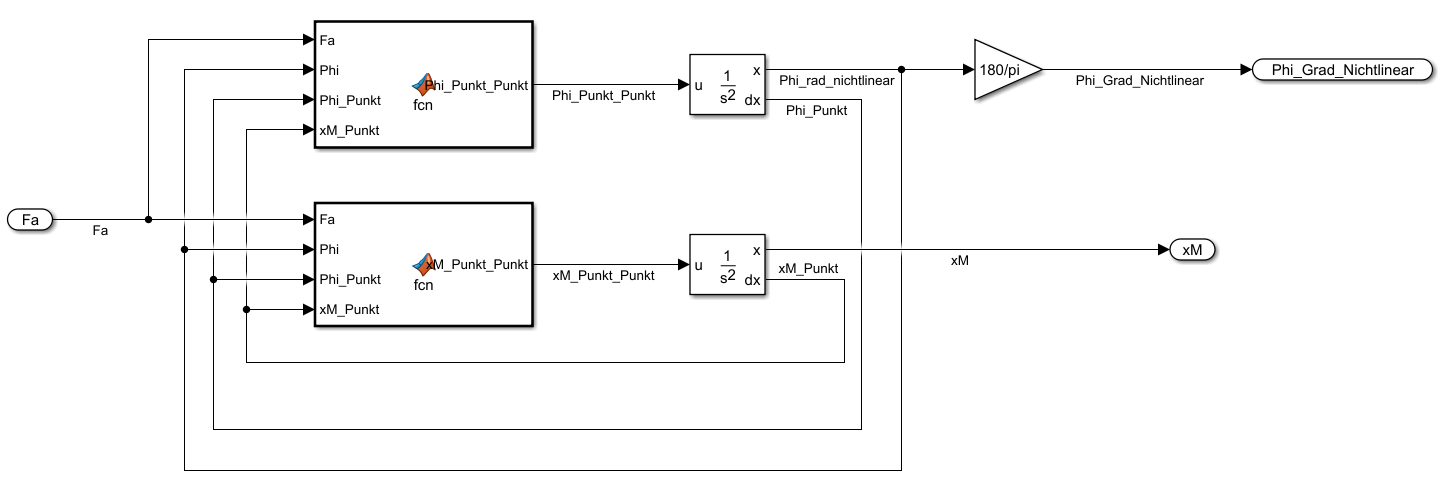
\includegraphics[width=0.85\textwidth]{Bilder/Simulinkmodell_nichtlinear.png}}
   \caption[Simulinkmodell des nichtlinearen Systems]{Simulinkmodell des nichtlinearen Systems}
   \label{fig:Bild2}
\end{figure}

\begin{figure}[H]
   \centering
   \fbox{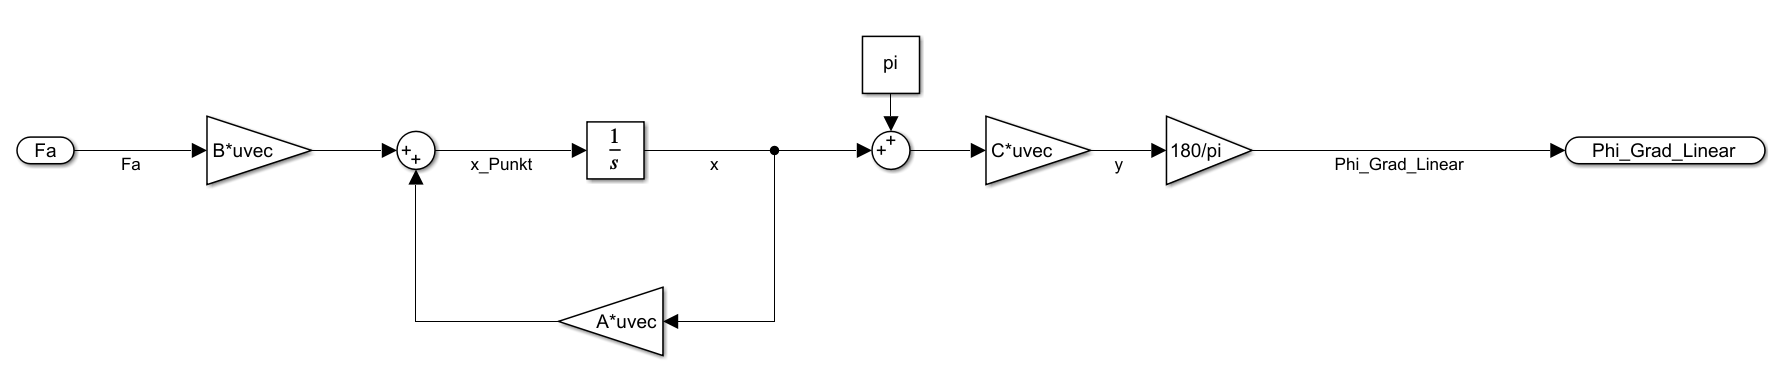
\includegraphics[width=0.85\textwidth]{Bilder/Simulinkmodell_linearisiert.png}}
   \caption[Simulinkmodell des linearisierten Systems]{Simulinkmodell des linearisierten Systems}
   \label{fig:Bild3}
\end{figure}

Beim Vergleich der beiden Systemverhalten ist zu erkennen, dass diese für kleine Winkelauslenkungen nahezu identsich erscheinen (\autoref{fig:Bild4} und \autoref{fig:Bild5}). Durch den sinusoidalen Signalverlauf wird weiter geschlussfolgert, dass eine positive Eingangskraft (Wagen fährt nach rechts) das Pendel in positive Winkelrichtung ausschlagen lässt. Da keine weiteren äußeren Kräfte auf das System eingeprägt werden, erfolgt mit steigender Zeit t durch die Reib- und Dämpfungsmomente das erneute Einpendeln in die stabile Ruhelage (hängendes Pendel).
\begin{figure}[H]
   \centering
   \fbox{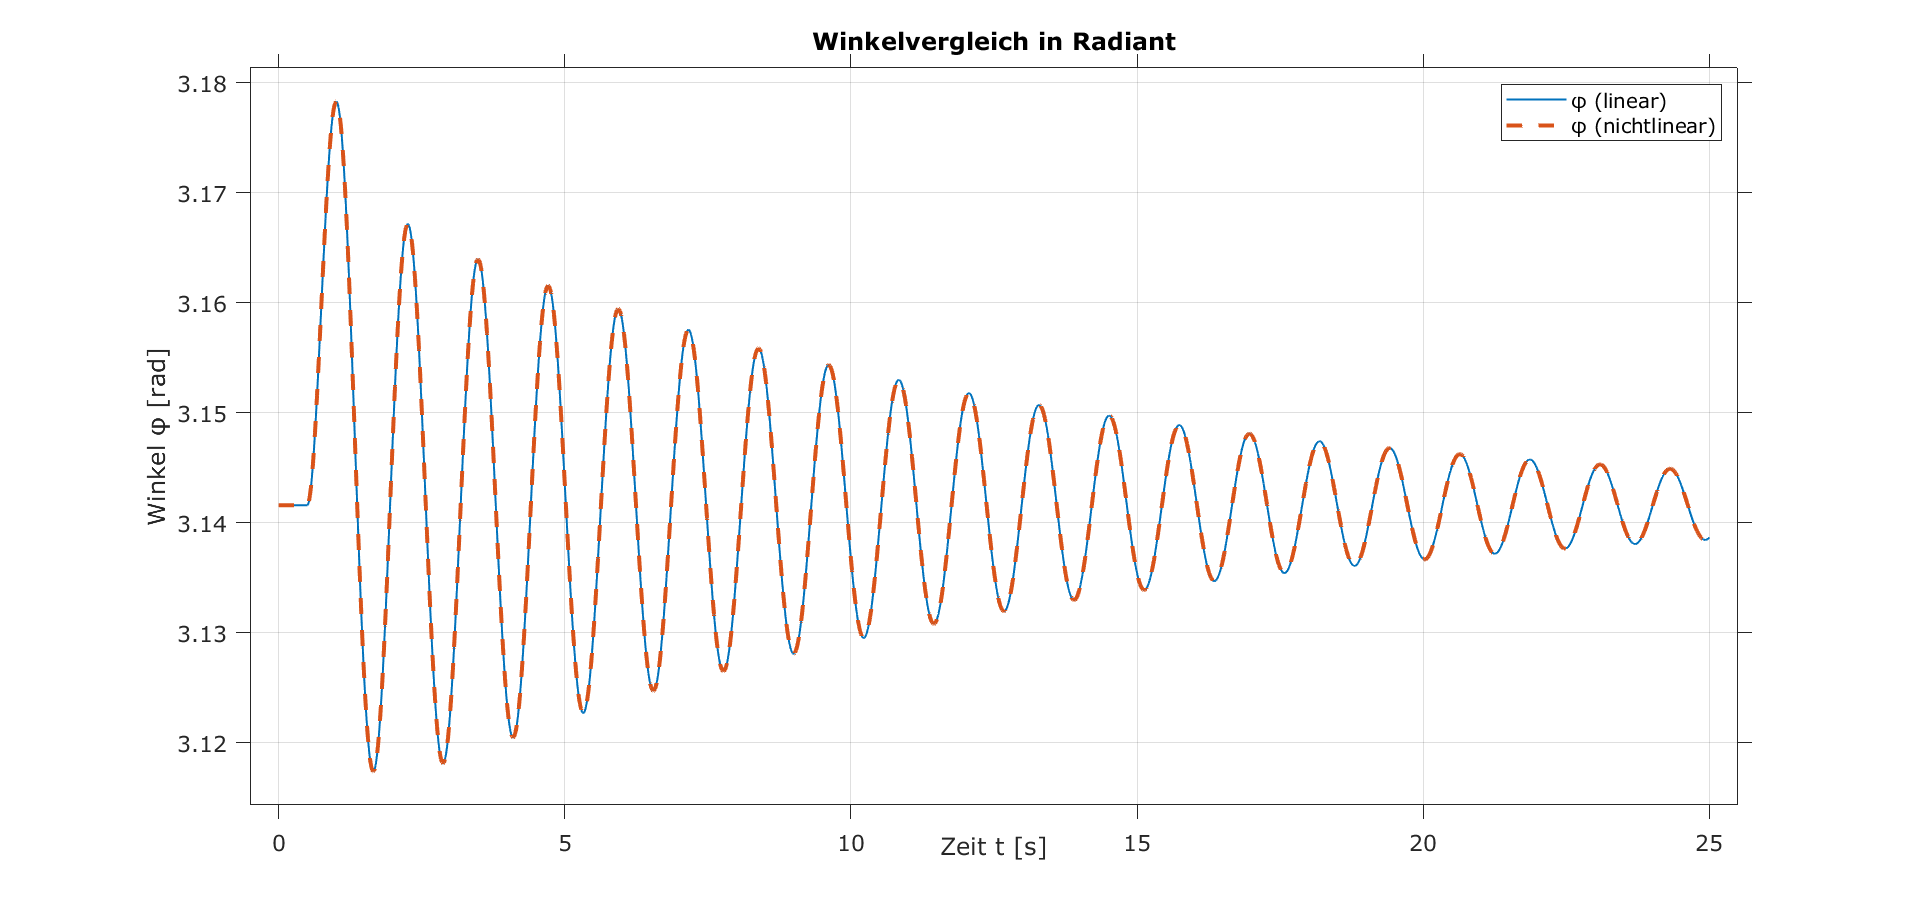
\includegraphics[width=0.9\textwidth]{Bilder/Phi_rad_Vergleich.png}}
   \caption[Vergleich der beiden radialen Winkelverläufe]{Vergleich der beiden radialen Winkelverläufe}
   \label{fig:Bild4}
\end{figure}
\begin{figure}[H]
    \centering
    \fbox{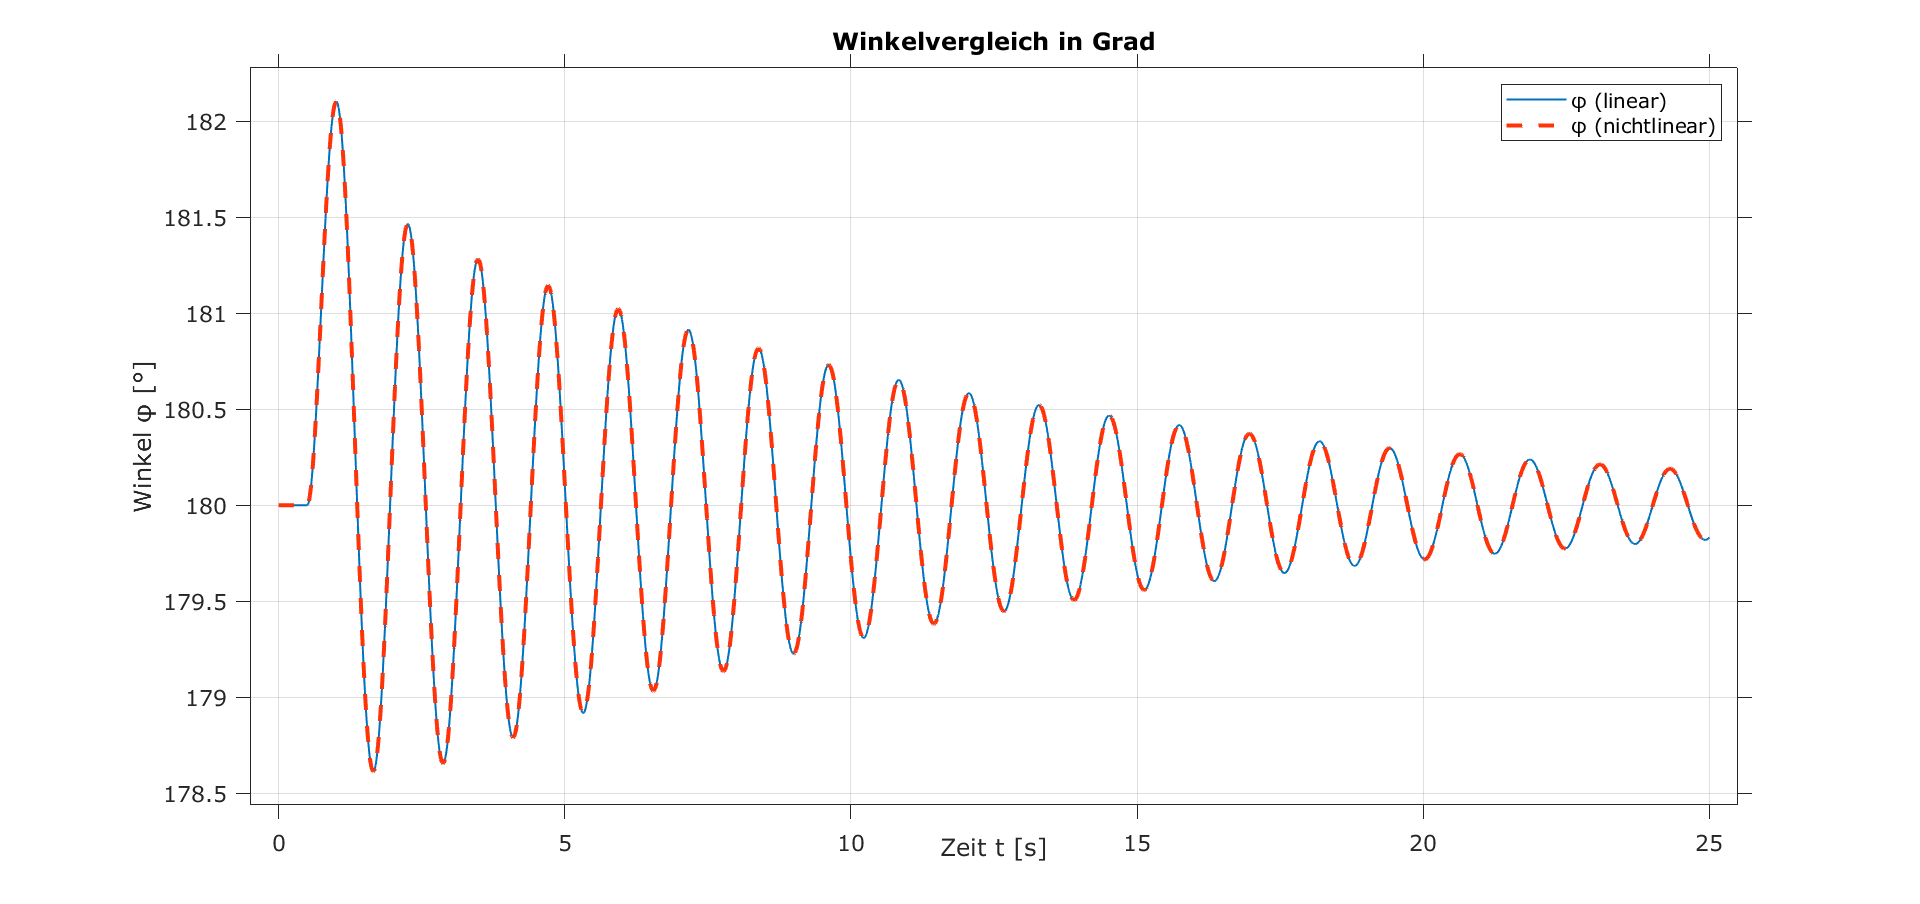
\includegraphics[width=0.9\textwidth]{Bilder/Phi_Grad_Vergleich.png}}
    \caption[Vergleich der beiden Winkelverläufe in Grad]{Vergleich der beiden Winkelverläufe in Grad}
    \label{fig:Bild5}
\end{figure}
Wird die Eingangkraft $F_{\mathrm{a}}$, welche auf das System wirkt, signifikant vergrößert (Einheitssprung mit Amplitude 15), werden größere Winkelauslenkungen erreicht. Dies führt zur Verringerung der Zuverlässigkeit des linearisierten Systems und zu Abweichungen zwischen dem linearen und nichtlinearem Systemverhalten (\autoref{fig:Bild6}).

\begin{figure}[H]
    \centering
    \fbox{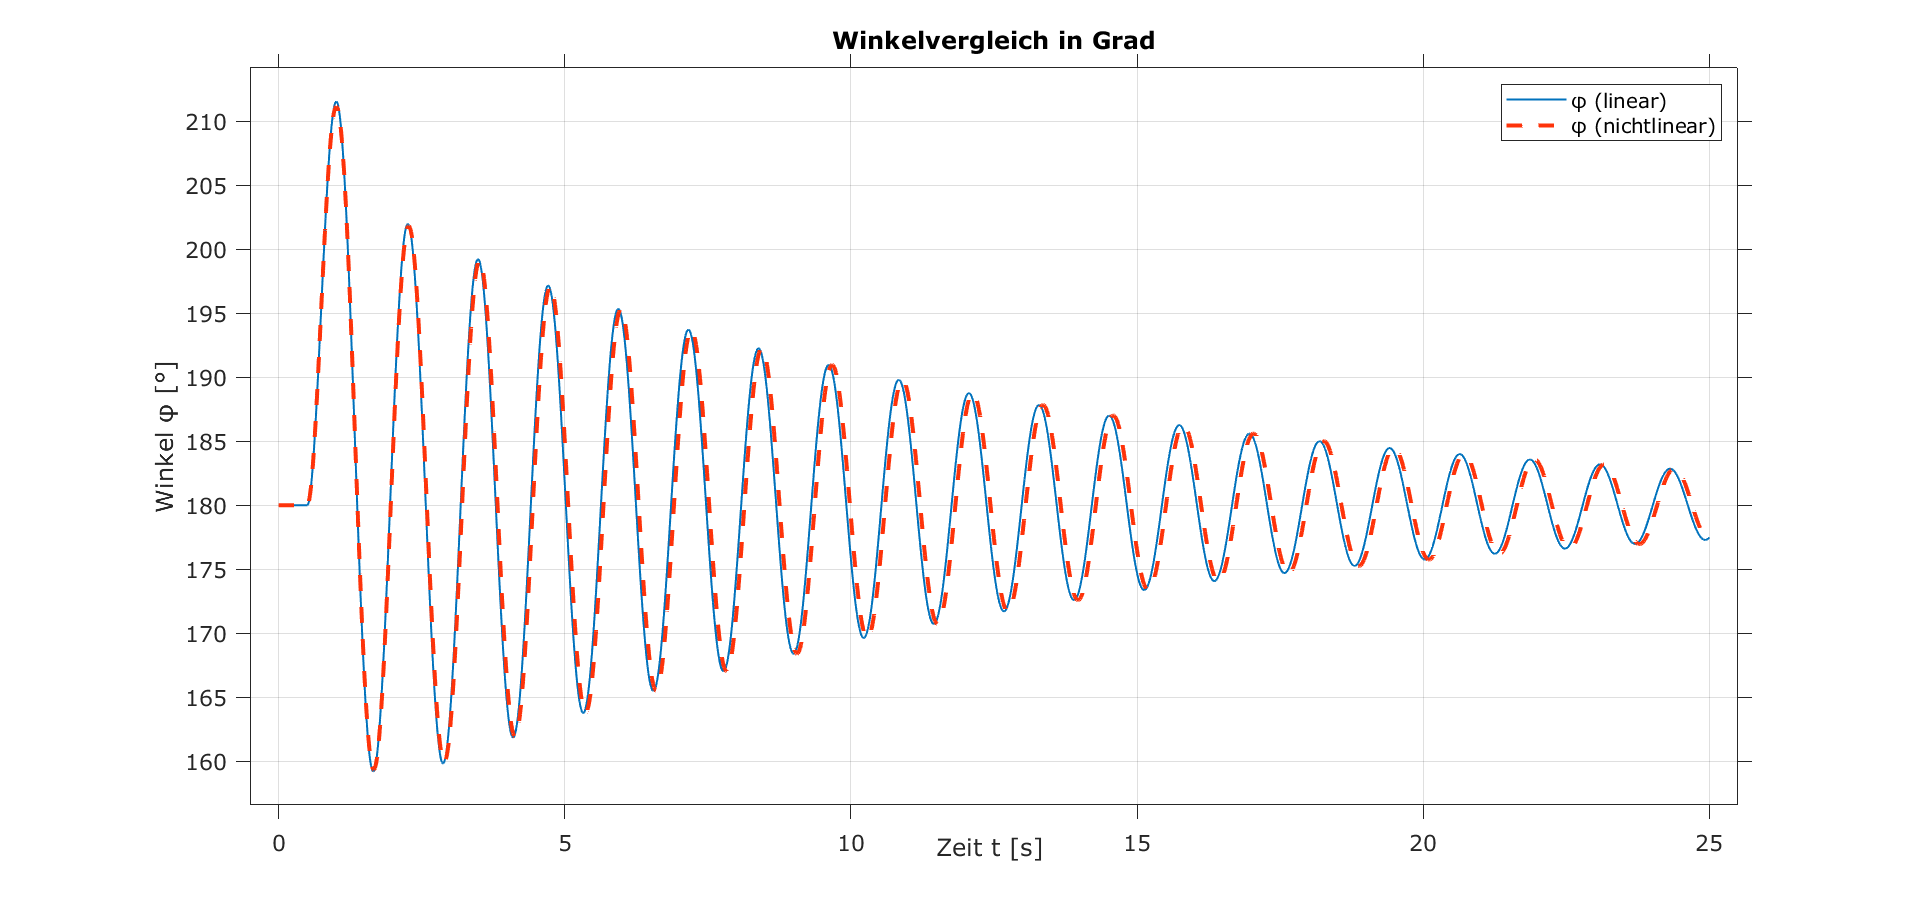
\includegraphics[width=0.9\textwidth]{Bilder/Phi_Grad_Vergleich_Verschiebung.png}}
    \caption[Vergleich der beiden Winkelverläufe in Grad mit Abweichung]{Abweichungen im Systemverhalten für größere Winkelauslenkungen}
    \label{fig:Bild6}
\end{figure}

\clearpage

\section{Zustandsreglerentwurf}

\subsection{Ackermann-Formel} \label{sec:Ackermann}

\begin{figure}[H]
    \centering
    \fbox{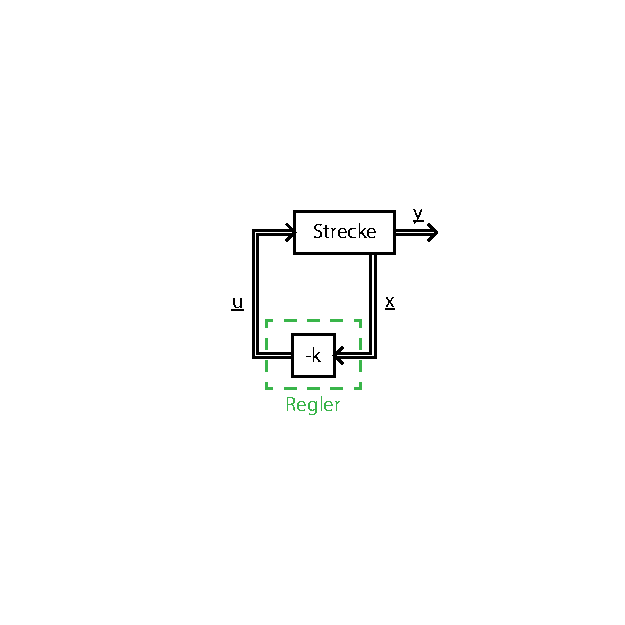
\includegraphics[width=0.3\textwidth]{Bilder/Ackermann.pdf}}
    \caption[Reglerstruktur Ackermann]{Schematische Darstellung der Reglerstruktur des Reglers mit Ackermann-Formel}
    \label{fig:Bild7}
\end{figure}

Die erste umgesetzte Regelstrategie ist die Anwendung der Ackermann-Formel. Ziel ist es das Pendel-System nach einem Impuls erneut in die instabile Ruhelage zu bringen. Dafür werden mit Hilfe der Ackermann-Formel die $"k"$-Faktoren berechnet, welche anschließend mit den Zuständen $x_{\mathrm{1}}$ bis $x_{\mathrm{4}}$ multipliziert und anschließend auf den Systemeingang zurückgeführt werden. Der Wagen wird dabei immer in den Ausgangszustand von $x_M$ zurück geregelt.\\

Im ersten Schritt wird der Nachweis der Steuerbarkeit des Systems benötigt. Dieser wurde bereits in \autoref{sec:Steuerbarkeit} erbracht.
Im zweiten Schritt erfolgt die Bestimmung der Eigenwerte der Systemmatrix A. Hierzu wird das charakteristische Polynom benötigt, welches mithilfe der Laplace-Transformation der Vektorzustandsdifferentialgleichungen $\underline{\dot{x}}$ und der anschließenden Umformung hergeleitet wird.\\\\
Laplace-Transformation und Umformung:
\begin{align*}
    \underline{\dot{x}} &= \underline{A}\cdot\underline{x}+\underline{B}\cdot\underline{u}\quad\laplace \quad s\cdot \underline{X}(s)-\underline{x}_{\mathrm{0}}=\underline{A}\cdot \underline{X}(s)+\underline{B}\cdot \underline{U}(s) \\
    \underline{X}(s) &= (s\cdot \underline{I} - \underline{A})^{-1}\cdot\underline{x}_{\mathrm{0}}+(s\cdot \underline{I} - \underline{A})^{-1}\cdot\underline{B}\cdot\underline{U}(s)
\end{align*}\\
Das charakteristische Polynom folgt aus der Determinante von: ($s\cdot\underline{I}-\underline{A}$). Die Matrix $\underline{I}$ stellt die Einheitsmatrix dar. Die Nullstellen des Polynoms gleichen der Eigenwerte der Systemmatrix A.\\\\
Charakteristische Polynom und Eigenwertdefinition:
\begin{align*}
    \underline{P}(s) &= det(s\cdot\underline{I}-\underline{A}) \\
    P(s_{\mathrm{P}}) &= 0 = eig(\underline{A})
\end{align*}

Allg. Form:
\begin{align*}
        \underline{P}(s) &= s^n+\alpha_{n-1}\cdot s^{\mathrm{n-1}}+...+\alpha_{\mathrm{1}}\cdot s + \alpha_{\mathrm{0}} \\
        \underline{P}(s) &= (s-s_{\mathrm{P1}})\cdot(s-s_{\mathrm{P1}})\cdot ... \cdot (s-s_{\mathrm{Pn}})
\end{align*}\\
Die Berechnung der Eigenwerte der Systemmatrix erfolgt analog zu den vorangegangenen Betrachtungen.\\\\
Eigenwerte des Systems:
\begin{align}
    eig(\underline{A}) &= eig
    \begin{bmatrix}
        0 & 1 & 0 & 0 \\
        26.6505 & -0.0248 & 0 & 5.8333 \\
        0 & 0 & 0 & 1 \\
        -0.8502 & 7.916\cdot10^-4 & 0 & -2.333
    \end{bmatrix} \nonumber\\
    eig(\underline{A}) &=
    \begin{bmatrix}
        0 \\
        -0.0914 + j 5.1281 \\
        -0.0914 - j 5.1281 \\
        -2.1753
    \end{bmatrix}
\end{align}\\
Die Eigenwerte müssen einen negativen Realteil aufweisen, andernfalls ist das System instabil. Zur Betrachtung des geregelten Systems, werden stabile Polstellen auf $s_{\mathrm{P}} = -1+0j$ festgelegt. Die Lage aller Polstellen ist in \autoref{fig:Bild7} visualisiert.\\\\
Wunschpolstellen:
\begin{align}
    \underline{s}_{\mathrm{P}} &= 
    \begin{bmatrix}
        -1 & -1 & -1 & -1 
    \end{bmatrix}
\end{align}
\begin{figure}[H]
    \centering
    \fbox{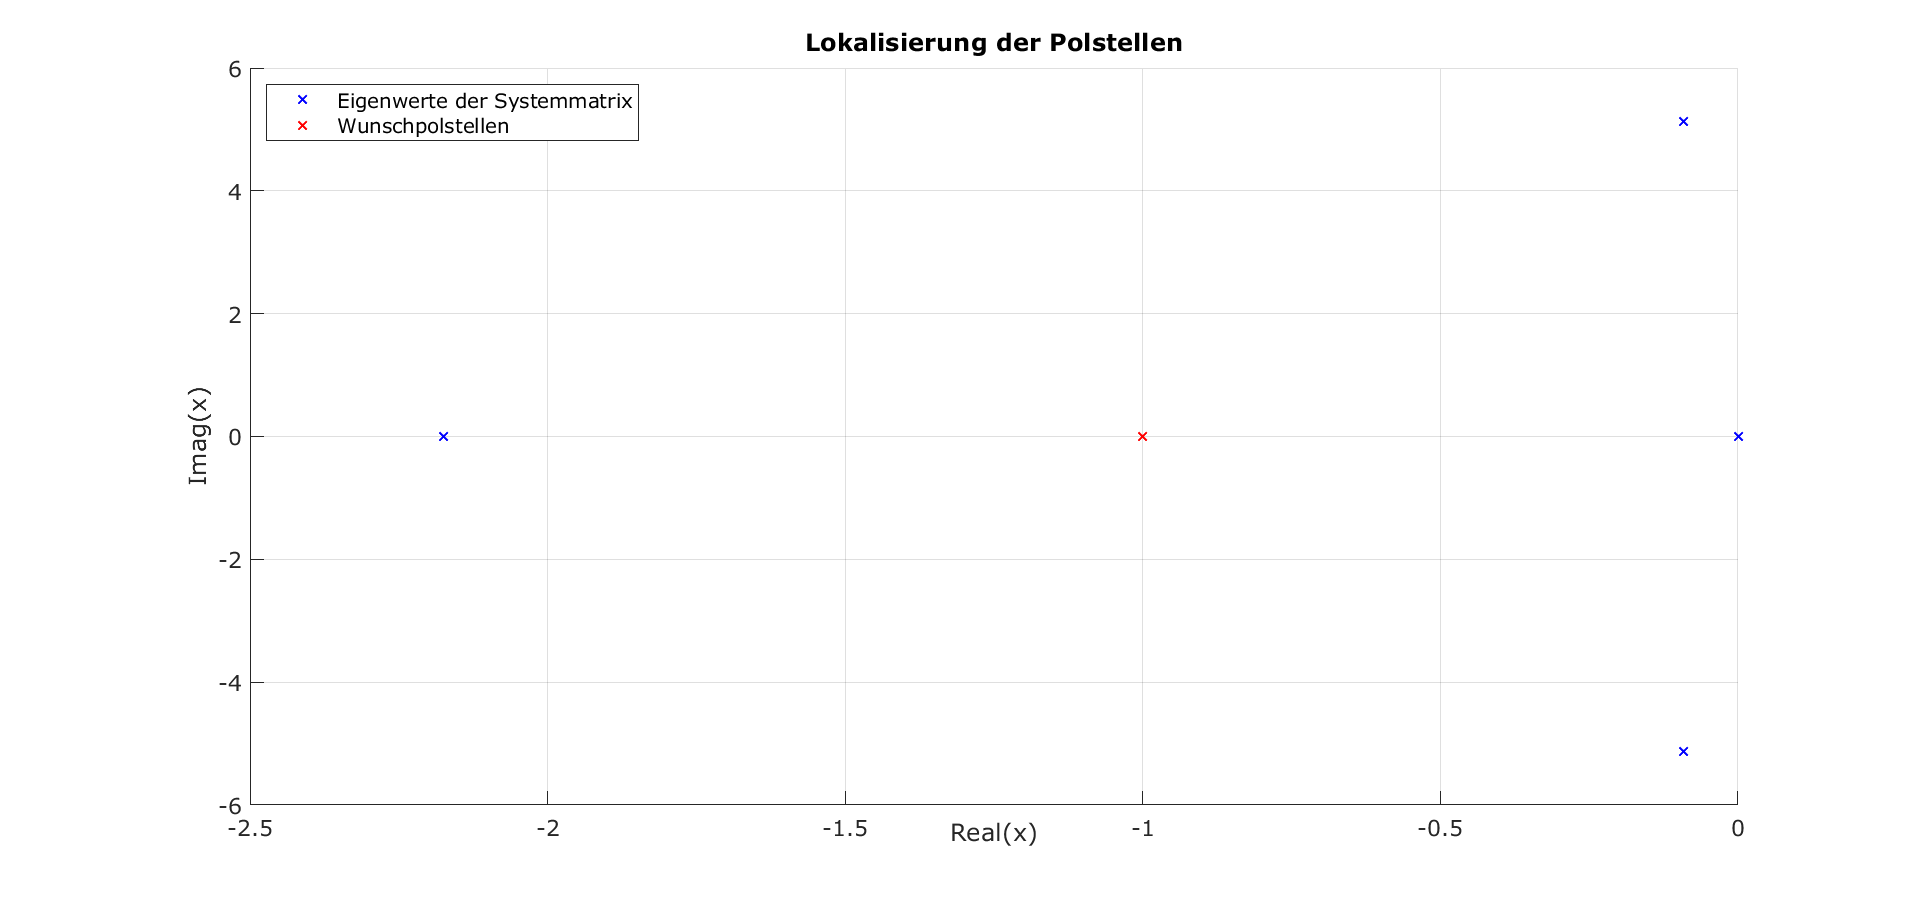
\includegraphics[width=0.9\textwidth]{Bilder/Polstellenlage.png}}
    \caption[Polstellenlage]{Polstellenlagen}
    \label{fig:Bild7}
\end{figure}

Zur Bestimmung der Koeffizienten $\alpha_{\mathrm{n}}$ bis $\alpha_{\mathrm{0}}$ des geregelten Systems, wird das charakteristische Polynom ausmultipliziert und die Wunschpolstellen eingesetzt.
Berechnung der Koeffizienten:
\begin{align*}
    \underline{P}(s) &= (s-s_{\mathrm{P1}})\cdot(s-s_{\mathrm{P2}})\cdot(s-s_{\mathrm{P3}})\cdot(s-s_{\mathrm{P4}}) \\
    \underline{P}(s) &= s^4-s^3\cdot(s_{\mathrm{P1}}+s_{\mathrm{P2}}+s_{\mathrm{P3}}+s_{\mathrm{P4}}) \nonumber \\ 
    &\quad +s^2\cdot(s_{\mathrm{P1}}\cdot(s_{\mathrm{P2}}+s_{\mathrm{P3}}+s_{\mathrm{P4}})+s_{\mathrm{P2}}\cdot(s_{\mathrm{P3}}+s_{\mathrm{P4}})+s_{\mathrm{P3}}\cdot s_{\mathrm{P4}}) \nonumber \\
    &\quad -s\cdot(s_{\mathrm{P1}}\cdot(s_{\mathrm{P2}}\cdot s_{\mathrm{P3}}+s_{\mathrm{P2}}\cdot s_{\mathrm{P4}}+s_{\mathrm{P3}}\cdot s_{\mathrm{P4}})+s_{\mathrm{P2}}\cdot s_{\mathrm{P3}}\cdot s_{\mathrm{P4}}) \nonumber \\
    &\quad +(s_{\mathrm{P1}}\cdot s_{\mathrm{P2}}\cdot s_{\mathrm{P3}}\cdot s_{\mathrm{P4}})
\end{align*}\\
Das charakteristische Polynom und die Koeffizienten folgen zu:
\begin{align}
    \underline{P}(s) &= s^4+4\cdot s^3+6\cdot s^2+4\cdot s+1 \nonumber \\
    \underline{\alpha} &=
    \begin{bmatrix}
        1 & 4 & 6 & 4 & 1
    \end{bmatrix} \label{eq:Gleichung38}
\end{align}\\
Zur Berechnung der Verstärkungsfaktoren des Reglers wird die letzte Zeile $t_{\mathrm{n}}^T$ der inversen Steuerbarkeitsmatrix $Q_{\mathrm{s}}^{-1}$ benötigt.\\\\
Inverse Steuerbarkeitsmatrix $Q_{\mathrm{s}}^{-1}$:
\begin{align*}
    \underline{Q}_{\mathrm{s}}^{-1} &=
    \begin{bmatrix}
         0 & -0.8333 & 1.9651 & -26.7984 \\
        -0.8333 & 1.9651 & -26.7984 & 67.7740 \\
        0 & 0.3333 & -0.7784 & 2.5264 \\
        0.3333 & -0.7784 & 2.5264 & -7.5869
    \end{bmatrix}^{-1} \\
    \underline{Q}_{\mathrm{s}}^{-1} &=
    \begin{bmatrix}
        0 & -0.1040 & 7 & 3.26 \\
        -0.1092 & -0.1142 & 3.2665 & 0.2854 \\
        -0.1165 & -0.0488 & 0.2885 & 0.1221 \\
        -0.0489 & 0 & 0.1223 & -0.0001
    \end{bmatrix}
\end{align*}\\
Letzte Zeile der inversen Matrix:
\begin{align} \label{eq:Gleichung39}
    \underline{t}_{\mathrm{4}}^T &=
    \begin{bmatrix}
        -0.0489 & 0 & 0.1223 & -0.0001
    \end{bmatrix}
\end{align}\\
Die finale Berechnung efolgt auf Grundlage der \autoref{eq:Gleichung40}. Durch das Einsetzen der letzten Zeile der inversen Steuerbarkeitsmatrix (\autoref{eq:Gleichung39}), der Faktoren aus \autoref{eq:Gleichung38} und der Systemmatrix A folgt für die Verstärkungsfaktoren $\underline{k}^T$:
\begin{align}
    \underline{k}^T &= \underline{t}_{\mathrm{n}}^T\cdot(\alpha_{\mathrm{0}}\cdot\underline{I} + \alpha_{\mathrm{1}}\cdot \underline{A} + ... + \alpha_{\mathrm{n-1}}\cdot \underline{A}^{n-1}+\underline{A}^n) \label{eq:Gleichung40}\\
    \underline{k}^T &=
    \begin{bmatrix}
        -24.8340 & 4.5745 & 0.1223 & -6.5108
    \end{bmatrix} \label{eq:Gleichung41}
\end{align}

\subsection{Vorsteuerung}

\begin{figure}[H]
    \centering
    \fbox{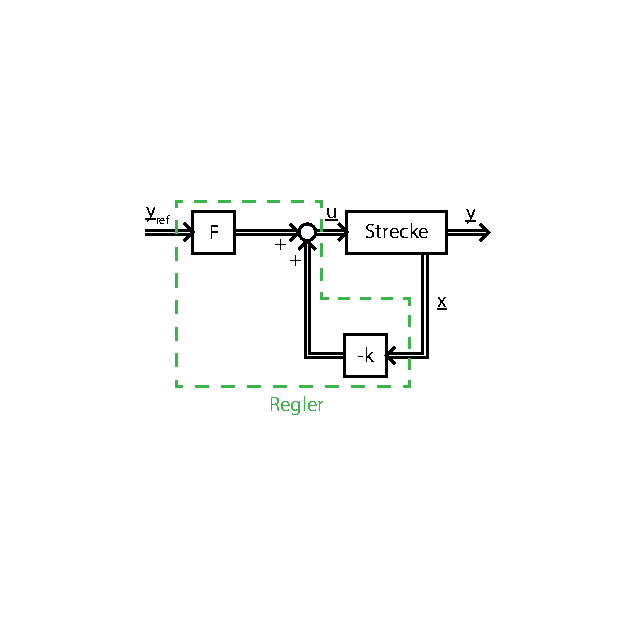
\includegraphics[width=0.5\textwidth]{Bilder/Vorsteuerung.pdf}}
    \caption[Reglerstruktur Vorsteuerung]{Schematische Darstellung der Reglerstruktur des Reglers mit Vorsteuerung}
    \label{fig:Bild8}
\end{figure}

Mithilfe des Vorfilters können andere Referenzpositionen des Wagens angesteuert werden, d.h. der Wagen fährt während des Pendelschwingens eine Endlage abweichend zum Ursprung an. Die Endlage wird mittels Referenzwert auf den Systemeingang gegeben. Dieser wird anschließend mit dem Vorfilter $\underline{F}$ multipliziert. Weiterhin erfolgt die Verrechnung mit den bereits in \autoref{sec:Ackermann} ermittelten Faktoren $\underline{k}$.\\\\
Eingangsgleichung des Systems:
\begin{align}\label{eq:Gleichung42}
    \underline{u}(t) &= -\underline{k}\cdot\underline{x}(t)+\underline{F}\cdot\underline{y}_{ref}(t)
\end{align}\\
Zur Ermittlung der Matrix $\underline{F}$ des Vorfilters werden zuerst die im Zeitbereich geltenden Kriterien aufgestellt. Der Ausgang des Systems $\underline{y}(t)$ muss nach unendlicher Zeit $t$ in den Referenzwert $\underline{y}_{ref}$ laufen. Der Referenzwert wird als konstant angenommen.\\\\
Kriterien im Zeitbereich:
\begin{align}
    \lim_{t \to \infty} \underline{y}(t) &= \underline{y}_{ref} = \underline{y}_{0ref} = const. \label{eq:Gleichung43}\\
    \underline{y}_{ref}(t) &=
    \begin{cases}
        \underline{y}_{0ref} & t \geq 0 \\
        0 & \, \text{sonst}
    \end{cases} \label{eq:Gleichung44}
\end{align}\\
Da die Berechnungen im Zeitbereich aufwendig sind, werden weitere Betrachtungen im Laplace-Bereich vorgenommen. Vorteil der Transformation ist das Rechnen mit algebraischen Gleichungen. Zur Überführung des Ansatzes aus \autoref{eq:Gleichung43} wird der Grenzwertsatz der Laplace-Transformation angewandt. Das Referenzzeitsignal $\underline{y}_{ref}(t)$ aus \autoref{eq:Gleichung44} wird ebenfalls überführt.\\\\
Grenzwertsatz der Laplace-Transformation und Überführung des Referenzzeitsignals:
\begin{align}
    \lim_{t \to \infty} \underline{y}(t) &= \lim_{s \to 0} s\cdot\underline{Y}(s) = \underline{y}_{ref} = \underline{y}_{0ref} \label{eq:Gleichung45}\\
    \underline{Y}_{ref}(s) &= \frac{1}{s}\cdot\underline{y}_{0ref} \label{eq:Gleichung46}
\end{align}\\
Für weitere Betrachtungen wird das Zustandsraummodell der Strecke in den Laplace-Bereich transformiert.\\\\
Laplace-Transformation der Strecke:
\begin{align}
    \underline{\dot{x}}(t) &= \underline{A}\cdot\underline{x}+\underline{B}\cdot\underline{u}(t)\quad\laplace\quad s\cdot \underline{X}(s) = \underline{A}\cdot\underline{X}(s)+\underline{B}\cdot\underline{U}(s) \label{eq:Gleichung47}\\
    \underline{y}(t) &= \underline{C}\cdot\underline{x}(t) \quad\laplace\quad \underline{Y}(s) = \underline{C}\cdot\underline{X}(s) \label{eq:Gleichung48}
\end{align}\\
Die \autoref{eq:Gleichung47} wird nach $\underline{X}(s)$ umgestellt und ensprechend in die Laplace-transformierte Ausgangsgleichung $\underline{Y}(s)$ eingesetzt. Aus der Umstellung geht hervor, dass das System durch eine Multiplikation aus einer Übertragungsfunktion $\underline{G}(s)$ und dem Eingangssignal $\underline{U}(s)$ gebildet werden kann.\\\\
Umformungen:
\begin{align}
    \underline{B}\cdot\underline{U}(s) &= (s\cdot\underline{I}-\underline{A})\cdot\underline{X}(s) \label{eq:Gleichung49}\\
    \underline{X}(s) &= (s\cdot\underline{I}-\underline{A})^{-1}\cdot\underline{B}\cdot\underline{U}(s) \nonumber \\
    \underline{Y}(s) &= \underline{C}\cdot(s\cdot\underline{I}-\underline{A})^{-1}\cdot\underline{B}\cdot\underline{U}(s) \label{eq:Gleichung50}\\
    \underline{G}(s) &= \underline{C}\cdot(s\cdot\underline{I}-\underline{A})^{-1}\cdot\underline{B} \nonumber
\end{align}\\
Die Eingangsgleichung des Systems (\autoref{eq:Gleichung42}) wird ebenfalls überführt und anschließend in \autoref{eq:Gleichung49} eingesetzt.\\\\
Laplace-Transformation der Eingangssgleichung:
\begin{align*}
    \underline{U}(s) &= -\underline{k}\cdot\underline{X}(s)+\underline{F}\cdot\underline{Y}_{\mathrm{ref}}(s)
\end{align*}\\
Einsetzen und Umformung nach $\underline{X}(s)$:
\begin{align}
    \underline{B}\cdot(\underline{F}\cdot\underline{Y}_{\mathrm{ref}}(s)-\underline{k}\cdot\underline{X}(s)) &= (s\cdot\underline{I}-\underline{A})\cdot\underline{X}(s) \nonumber \\
    \underline{B}\cdot \underline{F}\cdot\underline{Y}_{\mathrm{ref}}(s) &= (s\cdot\underline{I}-\underline{A}+\underline{B}\cdot{\underline{k}})\cdot\underline{X}(s) \nonumber \\
    \underline{X}(s) &= (s\cdot\underline{I}-\underline{A}+\underline{B}\cdot{\underline{k}})^{-1}\cdot\underline{B}\cdot \underline{F}\cdot\underline{Y}_{\mathrm{ref}}(s) \label{eq:Gleichung51}
\end{align}\\
Die \autoref{eq:Gleichung51} wird in \autoref{eq:Gleichung48} eingesetzt, um die Übertragungsfunktion des geschlossenen Regelkreises zu erhalten.\\\\
Übertragungsfunktion des geschlossenen Regelkreises:
\begin{align}
        \underline{Y}(s) &= \underline{C}\cdot(s\cdot\underline{I}-\underline{A}+\underline{B}\cdot{\underline{k}})^{-1}\cdot\underline{B}\cdot F\cdot\underline{Y}_{\mathrm{ref}}(s) \label{eq:Gleichung52}
\end{align}
Aus der vorangegangenen Betrachtung ist nur die Matrix $\underline{F}$ des Vorfilters unbekannt. Um dasjenige $F$ zu ermitteln, welches die stationäre Exaktheit erfüllt, wird der Grenzwertsatz aus \autoref{eq:Gleichung45} angesetzt und die Übertragungsfunktion des geschlossenen Regelkreises (\autoref{eq:Gleichung52}) eingesetzt.\\\\
Stationäre Exaktheit:
\begin{align}
    \lim_{s \to 0} s\cdot \underline{Y}(s) &= \underline{y}_{0ref} \nonumber \\
    \lim_{s \to 0} s\cdot (\underline{C}\cdot(s\cdot\underline{I}-\underline{A}+\underline{B}\cdot{\underline{k}})^{-1}\cdot\underline{B}\cdot\underline{F}\cdot\frac{1}{s}\cdot\underline{y}_{0ref}) &= \underline{y}_{0ref} \label{eq:Gleichung53}
\end{align}\\
Nach dem Vereinfachen der \autoref{eq:Gleichung53} geht hervor, dass der Term $\underline{C}\cdot(-\underline{A}+\underline{B}\cdot{\underline{k}})^{-1}\cdot\underline{B}\cdot\underline{F}$ der Einheitsmatrix $\underline{I}$ gleichen muss (\autoref{eq:Gleichung54}). Anderfalls ist die Gleichung nicht erfüllbar. Durch die Kenntnis kann die Matrix $\underline{F}$ des Vorfilters bestimmt werden (\autoref{eq:Gleichung55}).\\\\
Umstellung nach $\underline{F}$:
\begin{align}
    \underline{C}\cdot(-\underline{A}+\underline{B}\cdot{\underline{k}})^{-1}\cdot\underline{B}\cdot\underline{F} &= \underline{I} \label{eq:Gleichung54}\\
    \underline{F} = (\underline{C}\cdot(-\underline{A}+\underline{B}\cdot{\underline{k}})^{-1}\cdot\underline{B})^{-1} \label{eq:Gleichung55}
\end{align}\\
Die Anwendbarkeit des Reglergesetztes ist eingeschränkt, da nur quadratische Matrizen invertierbar sind. Die Dimensionen der einzelnen Matrizen lauten wie folgt:
\begin{itemize}
    \item $A\in\mathbb{R}^{(nxn)}$
    \item $B\in\mathbb{R}^{(nxm)}$
    \item $C\in\mathbb{R}^{(pxn)}$
    \item $k\in\mathbb{R}^{(mxn)}$
\end{itemize}
Die Matrix $\underline{F}$ ist quadratisch, sobald $p = m$ gilt, d.h. die Anzahl der Systemeingänge muss gleich der Anzahl der Systemausgänge sein.\\
Wird das linearisierte Zustandsraummodell (\autoref{eq:Gleichung33}) und die Faktoren $\underline{k}$ aus \autoref{eq:Gleichung41} in das Reglergesetz eingesetzt, resultiert der Faktor $F$ zu:\\
\begin{align}
    F &= 0.1223
\end{align}\\
Der Faktor $F$ ist ein skalarer Wert, da ein SISO-System vorliegt. Die Ausgangsmatrix $\underline{C}$ wurde entsprechend editiert, sodass die Wagenposition $x_{\mathrm{M}}$ als Systemausgang vorliegt: $\underline{C} = [0\quad0\quad1\quad0]$.

\subsection{I-Regelung}

\begin{figure}[H]
    \centering
    \fbox{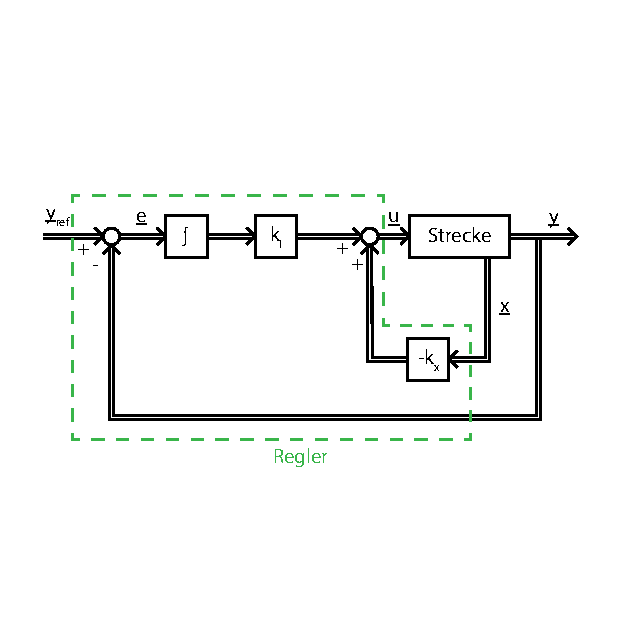
\includegraphics[width=0.7\textwidth]{Bilder/I-Regler.pdf}}
    \caption[Reglerstruktur I-Regelung]{Schematische Darstellung der Reglerstruktur des Reglers mit I-Regelung}
    \label{fig:Bild9}
\end{figure}

1. Reglergesetz:
\begin{align*}
    \underline{u} &= \underline{k}_{I}\cdot\int_{0}^t(\underline{y}_{ref}-\underline{y})d\tau-\underline{k}_{x}\cdot\underline{x}
\end{align*}
2. Definition:
\begin{align*}
    \underline{x}_{I}& :=\int_{0}^t(\underline{y}_{ref}-\underline{y})d\tau
\end{align*}
3. Einsetzen und Umformen
\begin{align*}
    \underline{u} &= \underline{k}_{I}\cdot\underline{x}_{I}-\underline{k}_{x}\cdot\underline{x} \\
    \underline{u} &= -\underline{k}_{x}\cdot\underline{x}+\underline{k}_{I}\cdot\underline{x}_{I}
\end{align*}
4. Tildevektoren
\begin{align*}
    \underline{u} &= -
    \begin{bmatrix}
        \underline{k}_{x} & -\underline{k}_{I}
    \end{bmatrix}
    \cdot
    \begin{bmatrix}
        \underline{x} \\
        \underline{x}_{I}
    \end{bmatrix} \\
    \underline{\tilde{k}} &= 
    \begin{bmatrix}
        \underline{k}_{x} & -\underline{k}_{I}
    \end{bmatrix} \\
    \underline{\tilde{x}} &= 
    \begin{bmatrix}
        \underline{x} \\
        \underline{x}_{I}
    \end{bmatrix}
\end{align*}
5. Vektor der Zustandsänderungen:
\begin{align*}
    \underline{\dot{x}}_{I} &= \frac{d}{dx}\cdot\int_{0}^t(\underline{y}_{ref}-\underline{y})d\tau = \underline{y}_{ref}-\underline{y} \\
    \underline{\dot{x}}_{I} &= \underline{y}_{ref}-\underline{C}\cdot\underline{x}
\end{align*}
6. Tildevektor der Zustände und Zustandsänderungen: 
\begin{align*}
    \underline{\dot{\tilde{x}}} &= 
    \begin{bmatrix}
        \underline{\dot{x}} \\
        \underline{\dot{x}}_{I}
    \end{bmatrix}\\
    \underline{\tilde{x}} &=
    \begin{bmatrix}
        \underline{x} \\
        \underline{x}_{I}
    \end{bmatrix}
\end{align*}
7. Ausgangsgleichung für erweitertes Zustandsraummodell:
\begin{align*}
    \underline{\dot{x}} &= \underline{A}\cdot\underline{x}+\underline{B}\cdot\underline{u} \\
    \underline{\dot{x}}_{I} &= \underline{y}_{ref}-\underline{C}\cdot\underline{x}
\end{align*}
8. Erweitertes Zustandsraummodell:
\begin{align*}
    \underline{\dot{\tilde{x}}} &= 
    \begin{bmatrix}
        \underline{A} & \underline{0} \\
        -\underline{C} & \underline{0}
    \end{bmatrix} \cdot \underline{\tilde{x}} +
    \begin{bmatrix}
        \underline{B} \\
        \underline{0}
    \end{bmatrix} \cdot\underline{u} +
    \begin{bmatrix}
        \underline{0} \\
        \underline{I}
    \end{bmatrix} \cdot\underline{y}_{ref}
\end{align*}
9. Resultierende Tildevektoren:
\begin{align*}
    \underline{\tilde{A}} &= 
    \begin{bmatrix}
        \underline{A} & \underline{0} \\
        -\underline{C} & \underline{0}
    \end{bmatrix} \\
    \underline{\tilde{B}} &= 
    \begin{bmatrix}
        \underline{B} \\
        \underline{0}
    \end{bmatrix} \\
    \underline{\tilde{B}}_{y} &= 
    \begin{bmatrix}
        \underline{0} \\
        \underline{I}
    \end{bmatrix}
\end{align*}


\clearpage

\section{Reglervalidierung}

\subsection{Validierung des linearen Modells}

Das Simulinkmodell der linearen Reglerstrecke ist in \autoref{fig:Bild3} dargestellt.

\subsubsection{Zustandsregler mit Ackermann-Formel}
% blockdiagramm des reglers

\begin{figure}[H]
    \centering
    \fbox{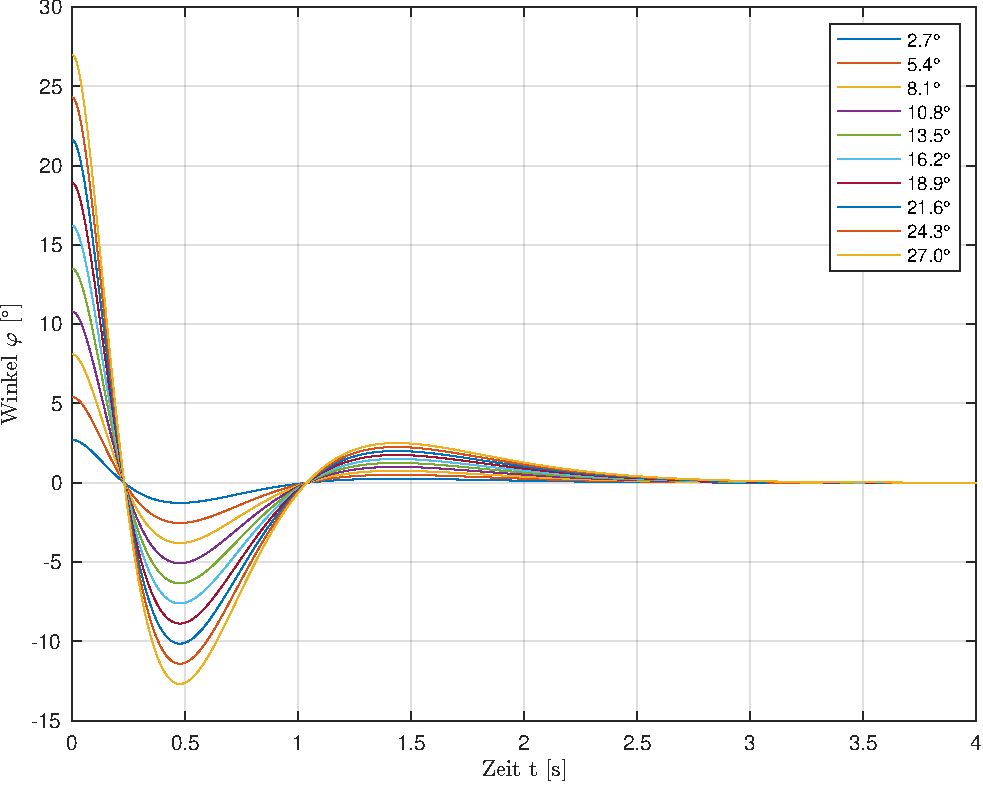
\includegraphics[width=0.6\textwidth]{Bilder/Reglervalidierung/linear_ackermann_phi.pdf}}
    \caption[$\varphi$ für Regler mit Ackermann-Formel]{$\varphi$ für verschiedene Anfangsauslenkungen am Zustandsregler mit Ackermann-Formel}
    \label{fig:Bild12}
\end{figure}

\begin{figure}[H]
    \centering
    \fbox{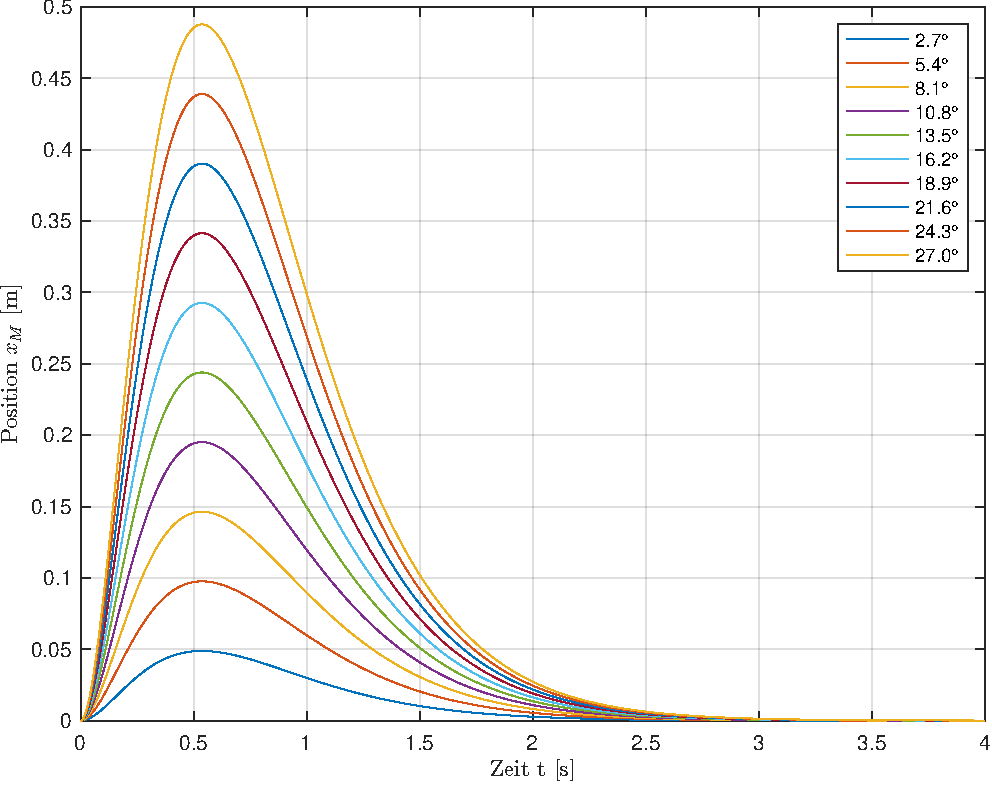
\includegraphics[width=0.6\textwidth]{Bilder/Reglervalidierung/linear_ackermann_xM.pdf}}
    \caption[$x_{\mathrm{M}}$ für Regler mit Ackermann-Formel]{$x_{\mathrm{M}}$ für verschiedene Anfangsauslenkungen am Zustandsregler mit Ackermann-Formel}
    \label{fig:Bild13}
\end{figure}

\begin{figure}[H]
    \centering
    \fbox{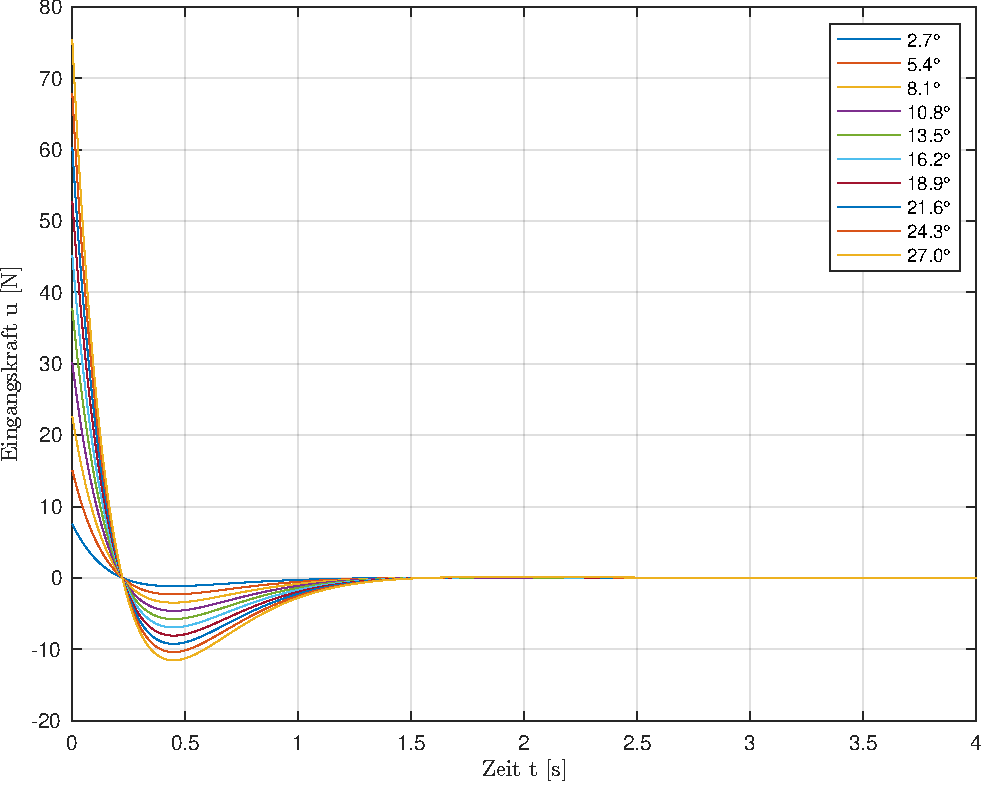
\includegraphics[width=0.6\textwidth]{Bilder/Reglervalidierung/linear_ackermann_u.pdf}}
    \caption[u für Regler mit Ackermann-Formel]{u für verschiedene Anfangsauslenkungen am Zustandsregler mit Ackermann-Formel}
    \label{fig:Bild14}
\end{figure}

\subsubsection{Zustandsregler mit Vorsteuerung}
% blockdiagramm des reglers

\begin{figure}[H]
    \centering
    \fbox{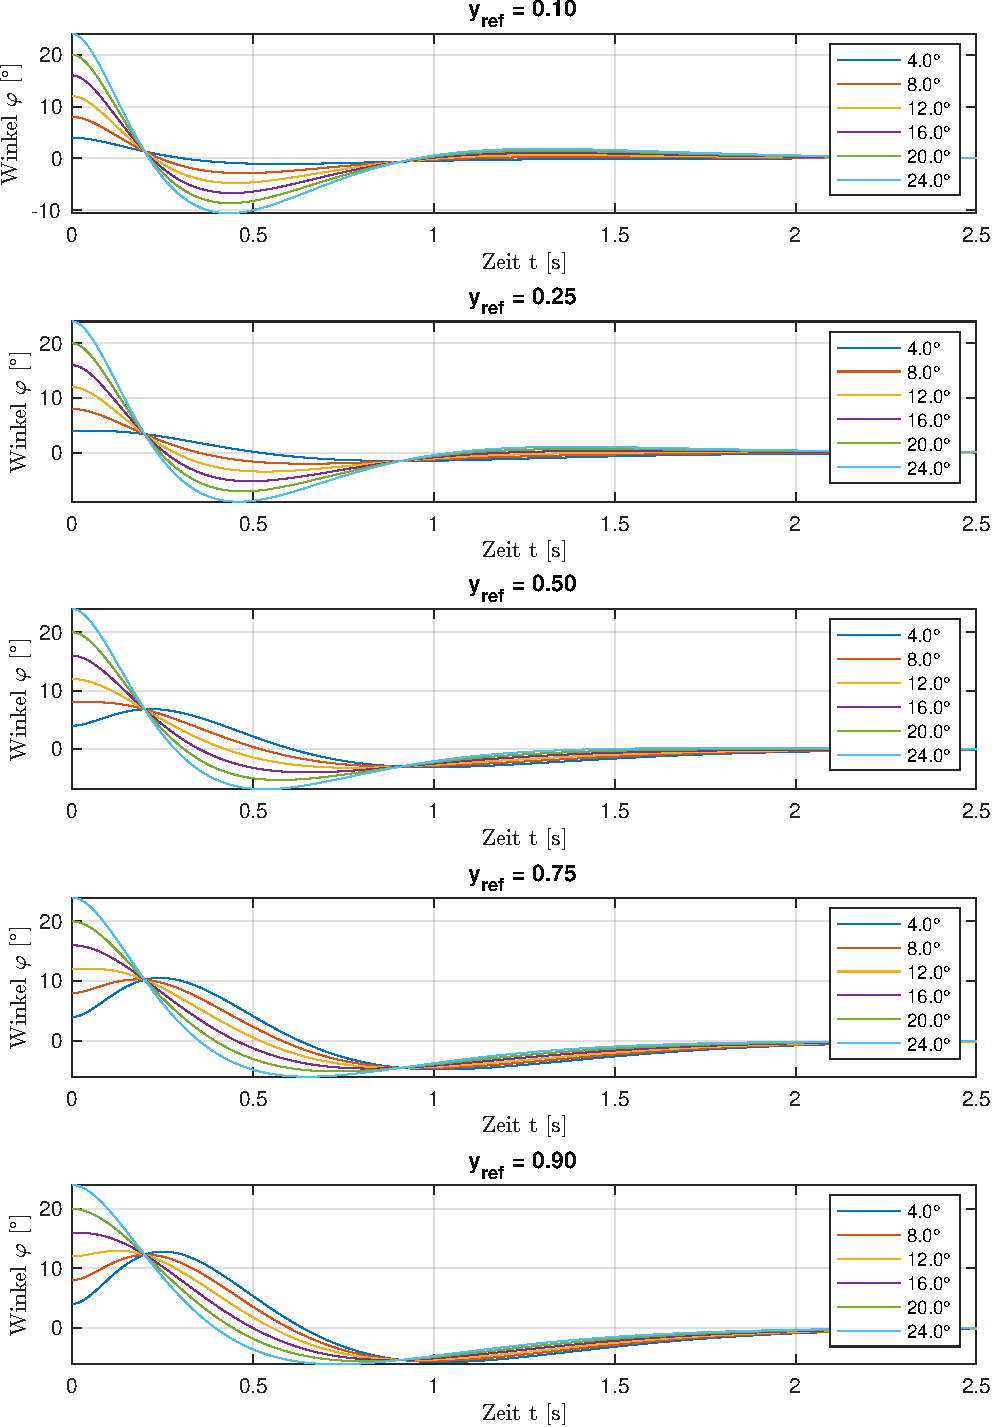
\includegraphics[width=0.76\textwidth]{Bilder/Reglervalidierung/linear_vorsteuerung_phi.pdf}}
    \caption[$\varphi$ für Regler mit Vorsteuerung]{$\varphi$ für verschiedene Referenzpositionen $y_{ref}$ und Anfangsauslenkungen am Zustandsregler mit Vorsteuerung}
    \label{fig:Bild15}
\end{figure}

\begin{figure}[H]
    \centering
    \fbox{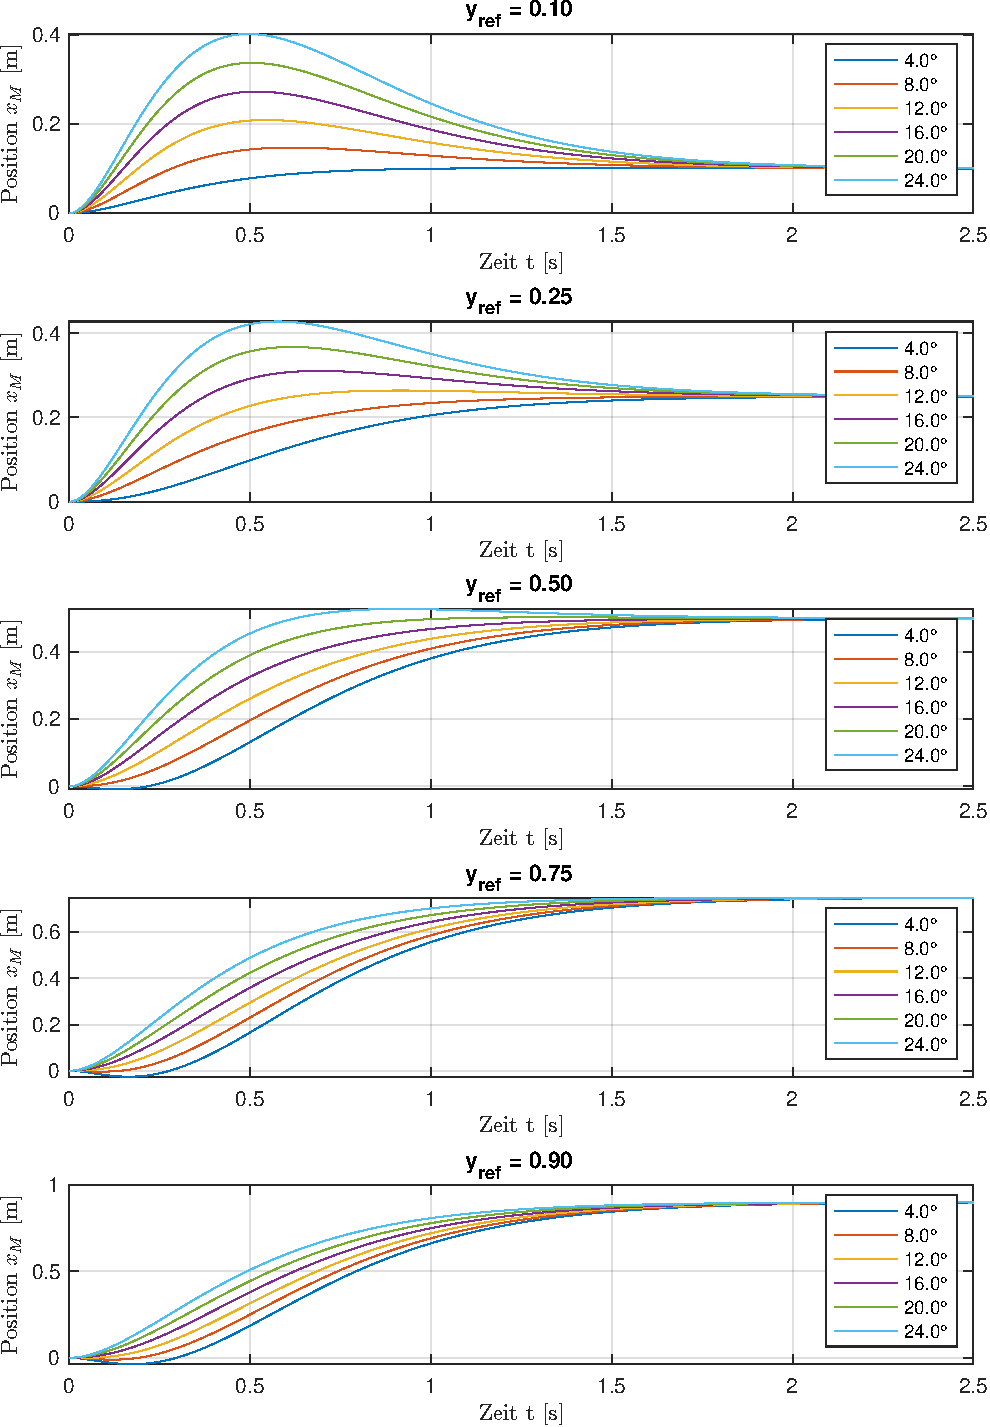
\includegraphics[width=0.8\textwidth]{Bilder/Reglervalidierung/linear_vorsteuerung_xM.pdf}}
    \caption[$x_{\mathrm{M}}$ für Regler mit Vorsteuerung]{$x_{\mathrm{M}}$ für verschiedene Referenzpositionen $y_{ref}$ und Anfangsauslenkungen am Zustandsregler mit Vorsteuerung}
    \label{fig:Bild16}
\end{figure}

\begin{figure}[H]
    \centering
    \fbox{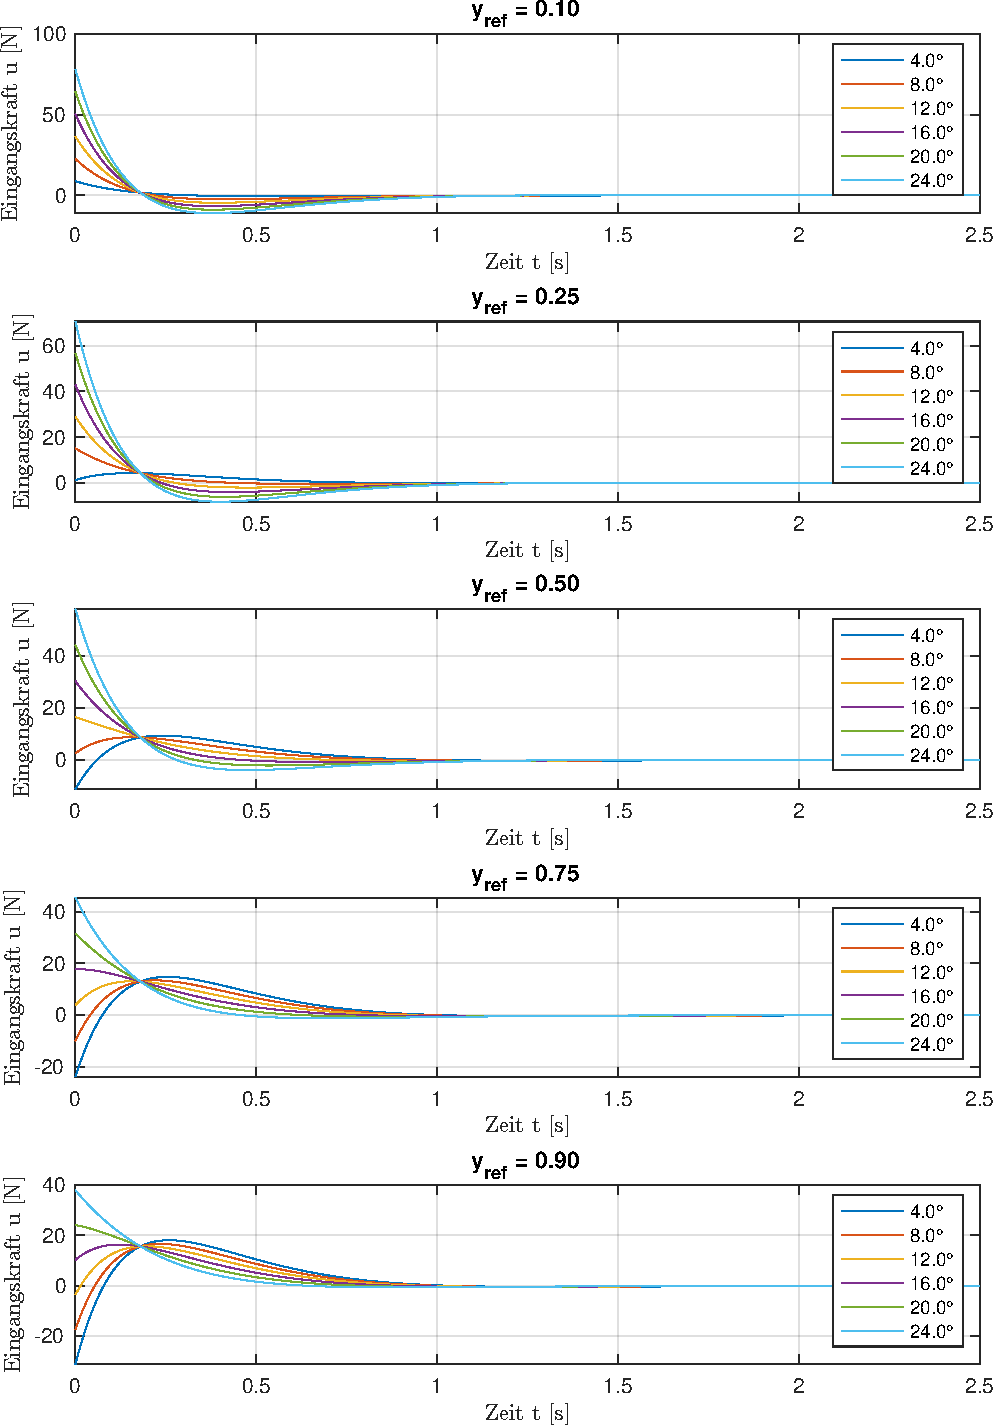
\includegraphics[width=0.8\textwidth]{Bilder/Reglervalidierung/linear_vorsteuerung_u.pdf}}
    \caption[u für Regler mit Vorsteuerung]{u für verschiedene Referenzpositionen $y_{ref}$ und Anfangsauslenkungen am Zustandsregler mit Vorsteuerung}
    \label{fig:Bild17}
\end{figure}

\subsubsection{Zustandsregler mit I-Regelung}
% blockdiagramm des reglers

\begin{figure}[H]
    \centering
    \fbox{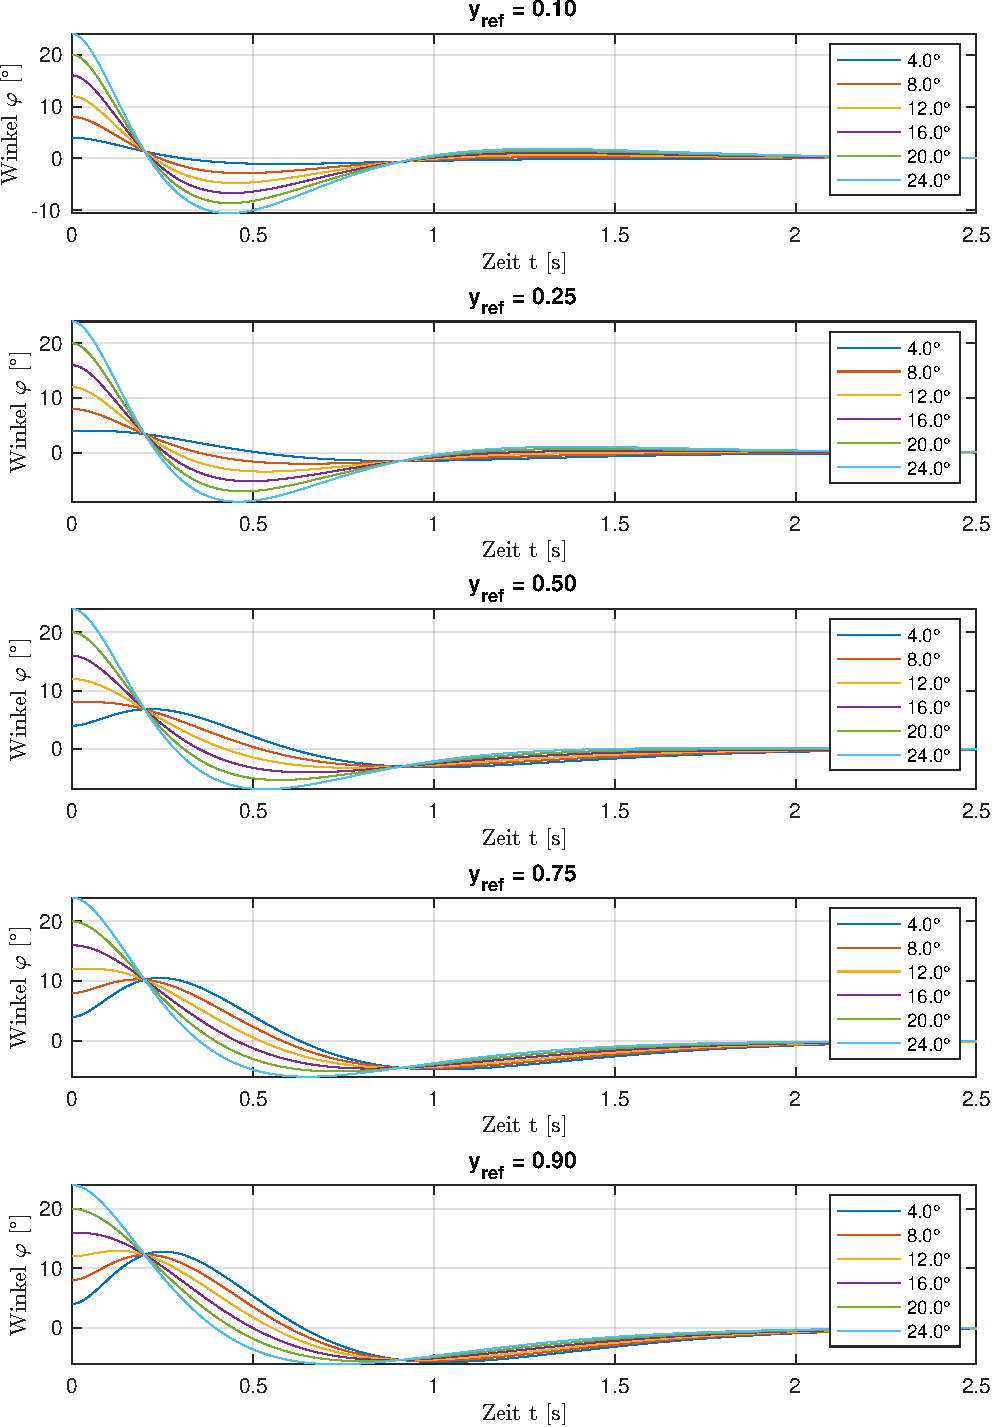
\includegraphics[width=0.76\textwidth]{Bilder/Reglervalidierung/linear_vorsteuerung_phi.pdf}}
    \caption[$\varphi$ für Regler mit I-Regelung]{$\varphi$ für verschiedene Referenzpositionen $y_{ref}$ und Anfangsauslenkungen am Zustandsregler mit I-Regelung}
    \label{fig:Bild18}
\end{figure}

\begin{figure}[H]
    \centering
    \fbox{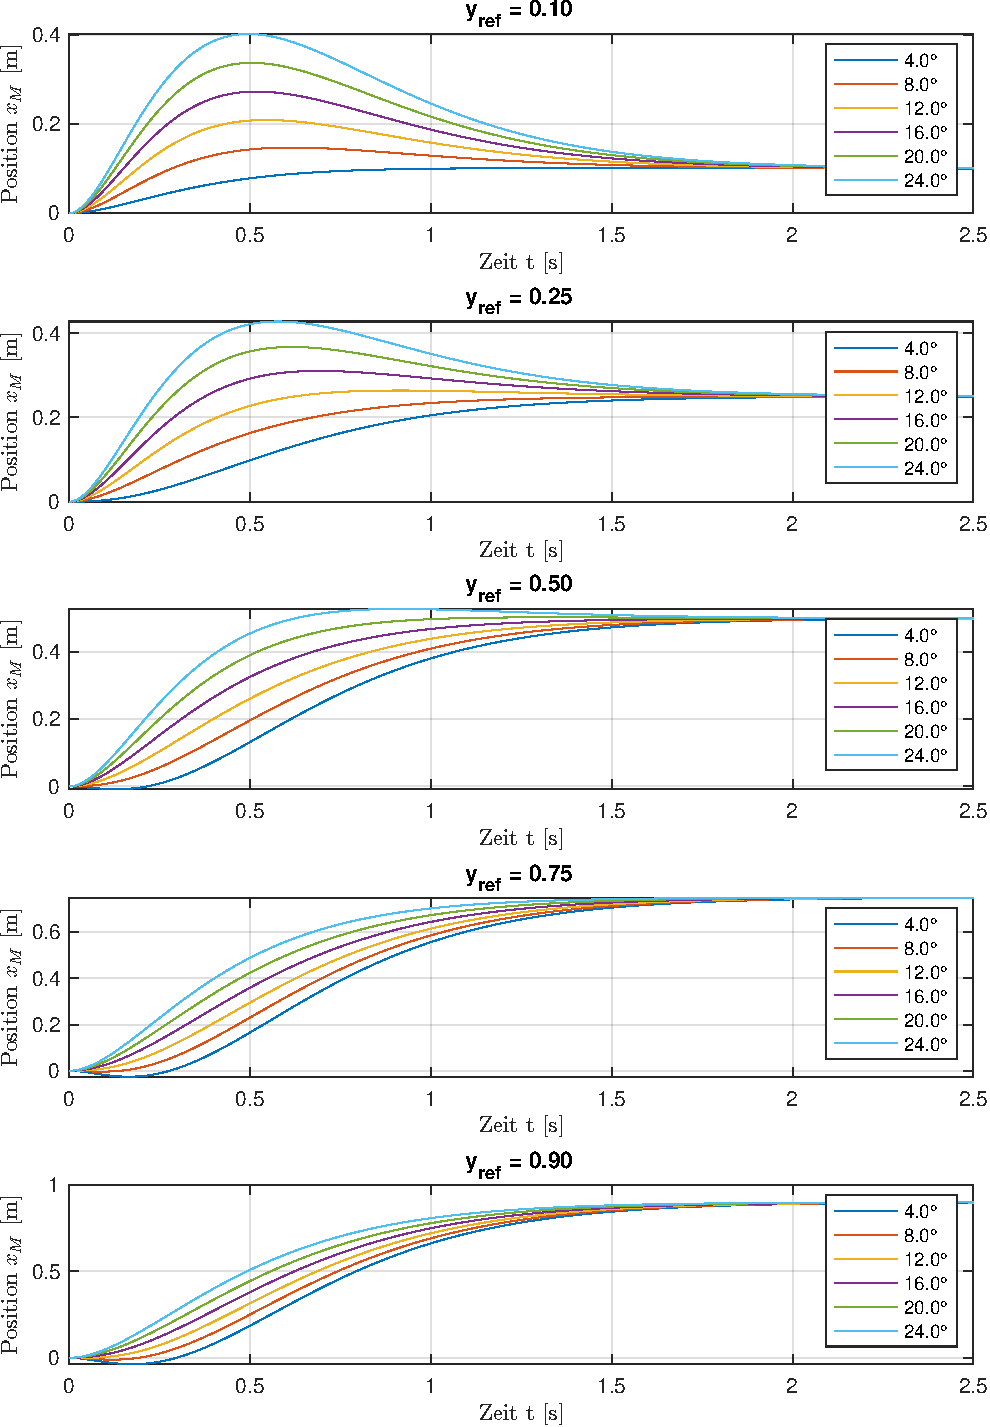
\includegraphics[width=0.8\textwidth]{Bilder/Reglervalidierung/linear_vorsteuerung_xM.pdf}}
    \caption[$x_{\mathrm{M}}$ für Regler mit I-Regelung]{$x_{\mathrm{M}}$ für verschiedene Referenzpositionen $y_{ref}$ und Anfangsauslenkungen am Zustandsregler mit I-Regelung}
    \label{fig:Bild19}
\end{figure}

\begin{figure}[H]
    \centering
    \fbox{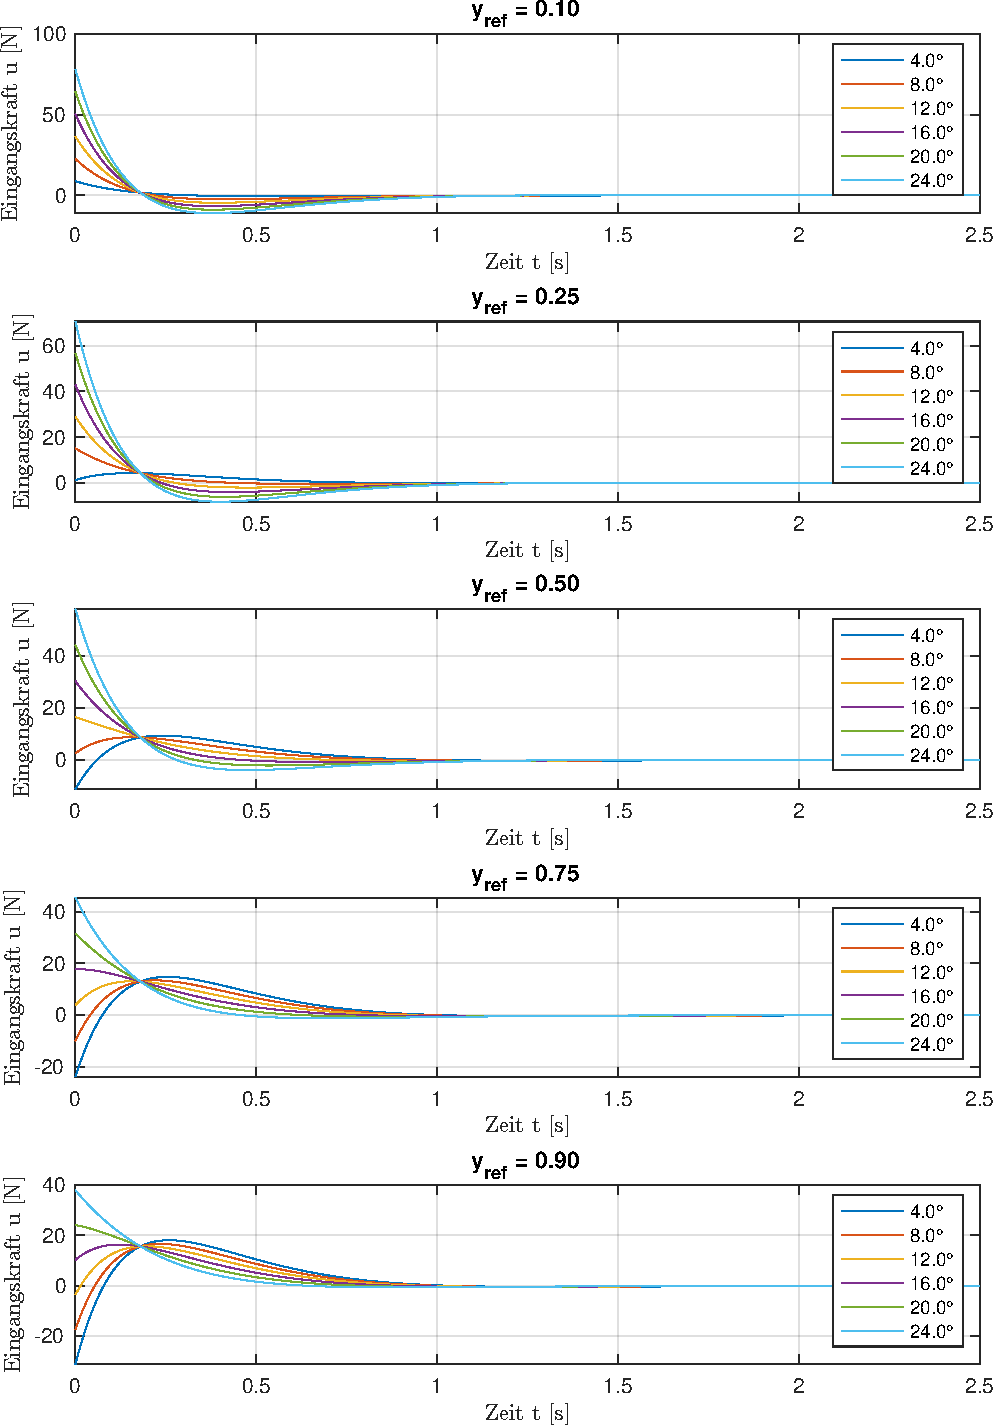
\includegraphics[width=0.8\textwidth]{Bilder/Reglervalidierung/linear_vorsteuerung_u.pdf}}
    \caption[u für Regler mit I-Regelung]{u für verschiedene Referenzpositionen $y_{ref}$ und Anfangsauslenkungen am Zustandsregler mit I-Regelung}
    \label{fig:Bild20}
\end{figure}

\subsubsection{Vergleich des Regelverhaltens}
% möglichst alle übereinander

\subsection{Validierung des nicht-linearen Modells}
% analog zu linear

Das Simulinkmodell der nicht-linearen Reglerstrecke ist in \autoref{fig:Bild2} dargestellt.

\subsubsection{Zustandsregler mit Ackermann-Formel}

\subsubsection{Zustandsregler mit Vorsteuerung}

\subsubsection{Zustandsregler mit I-Regelung}

\subsubsection{Vergleich des Regelverhaltens}

\clearpage

\section{Beobachtbarkeit}

\subsection{Überprüfung der Beobachtbarkeit}

\subsection{Beobachterentwurf}

\subsection{Beobachtervalidierung}

%---------Quellen---------------------------------
\newpage
\newcount\Quellennummer
\Quellennummer=1

\renewcommand\refname{Literaturverzeichnis}
\addcontentsline{toc}{section}{Literaturverzeichnis}

\begin{thebibliography}{999}
{\setlength{\emergencystretch}{3cm}%

\bibitem[\the\Quellennummer]{HTWgross}
HTW-Logo auf dem Deckblatt\par
\url{https://de.wikipedia.org/wiki/Datei:Logo_HTW_Berlin.svg} \par
 Stand: 17.08.2018 um 14:49 Uhr

\advance\Quellennummer by 1
 
\bibitem[\the\Quellennummer]{HTWklein}
HTW-Logo in der Kopfzeile\par
\url{http://tonkollektiv-htw.de/} \par
 Stand: 17.08.2018 um 14:53 Uhr

\advance\Quellennummer by 1

\bibitem[\the\Quellennummer]{SkriptSchulte}
Skript Moderne Methoden der Regelungstechnik\par
Prof.\xspace Dr.\xspace -Ing.\xspace Horst Schulte

\advance\Quellennummer by 1

\bibitem[\the\Quellennummer]{LinBrandstaedter}
Anleitung Linearisierung eines zeitinvarianten,\par
nichtlinearen Zustandmodells\par
Prof.\xspace Dr.\xspace -Ing.\xspace Heide Brandstädter

\advance\Quellennummer by 1

\bibitem[\the\Quellennummer]{RegelungBuss}
Regelungs- und Steuerungstechnik: Polstellenverteilung\par
Prof.\xspace Dr.\xspace -Ing.\xspace M. Buss

\advance\Quellennummer by 1

}
\end{thebibliography}

\end{document}
